\documentclass[twocolumn]{article}
\usepackage{amsmath, amssymb, graphicx, siunitx}
\title{Direct Tests of a Pixelated Microchannel Plate as the Active Element of a Shower Maximum Detector}

\author{Federico Presutti
\and Mentor: M. Spiropulu
\and Co-Mentor: Artur Apresyan, Si Xie, Cristian Pena}

\begin{document}

\twocolumn[
\begin{@twocolumnfalse}
\maketitle

\begin{abstract}
One possibility to make a fast and radiation resistant shower maximum detector is to use a secondary emitter as an active element. We further the study of microchannel plate photomultipliers (MCPs) as an active element of a shower-maximum detector. We present test beam results obtained using Photonis XP85011 and Photek 240 MCPs to detect secondary particles of an electromagnetic shower. We focus on the use of the multiple pixels on the Photonis MCP in order to find a transverse two-dimensional shower maxima distribution. A spatial resolution of 0.8 mm was obtained with an 8 GeV electron beam. A method for measuring time resolution from the Photonis MCP as a whole is presented, and it improves the time resolution for individual pixel readouts. The time resolution is found to be better than 40 ps.
\end{abstract}

\end{@twocolumnfalse}
]



\title{\large}{\textbf{Introduction}}

A calorimetric technique that is used for the detection of high energy particles involves the use of a dense material that causes the particles to shower. When a particle showers it generates secondary particles of lesser energy. The number of secondary particles at a given shower depth is proportional to the energy of the initial incoming particle. The energy deposited is then measured by an active component in the calorimeters, usually a photomultiplier of some variety.

It would be advantageous for future high-energy physics experiments to have working shower-maximum detectors and calorimeters with improved timing properties and with virtually infinite radiation hardness.

A recent candidate device with very high time resolution are microchannel-plate detectors (MCPs). An advantage of these devices other than their timing properties is that they can be pixelated -- separated into multiple individual channels. This is the case for the Photonis XP85011 MCP. This is an attractive property since it is possible to obtain a two-dimensional map of energy, and thus can be used as shower-maxima detectors, whose purpose is to find the center of the particle shower following the impact of a high-energy particle. There is an impact on the timing performance of the pixelated MCP when considering individual channels compared to compounding them into one larger-aperture channel. Nonetheless, the time resolution we obtained on the Photonis XP85011 was on the order of \SI{40}{\pico\second} and the spatial resolution as a shower-maximum detector was on the order of \SI{1}{\milli\meter}.

\begin{figure}[htbp]
	\centering
	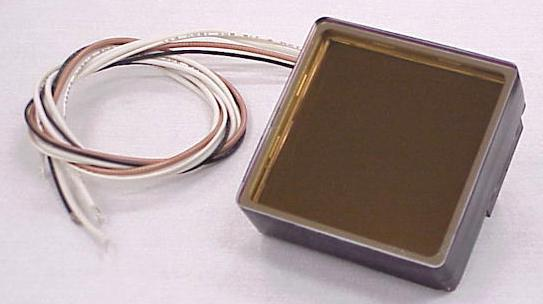
\includegraphics[width=8cm]{Images/photonis/photonis.jpg}
	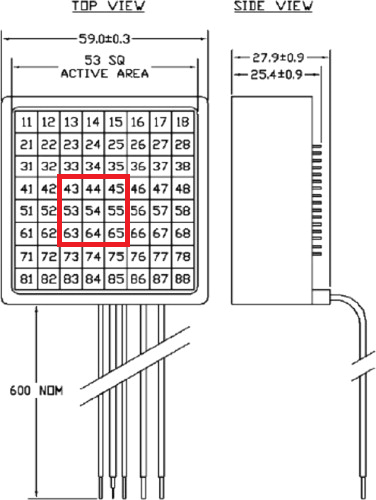
\includegraphics[width=8cm]{Images/photonis/photonis2.png}
	\caption{\small External view of the Photonis XP85011 MCP and schematic. The red box indicates the selection of pixels used in this experiment.}
	\label{fig:photonis}
\end{figure}

\begin{figure}[htbp]
	\centering
	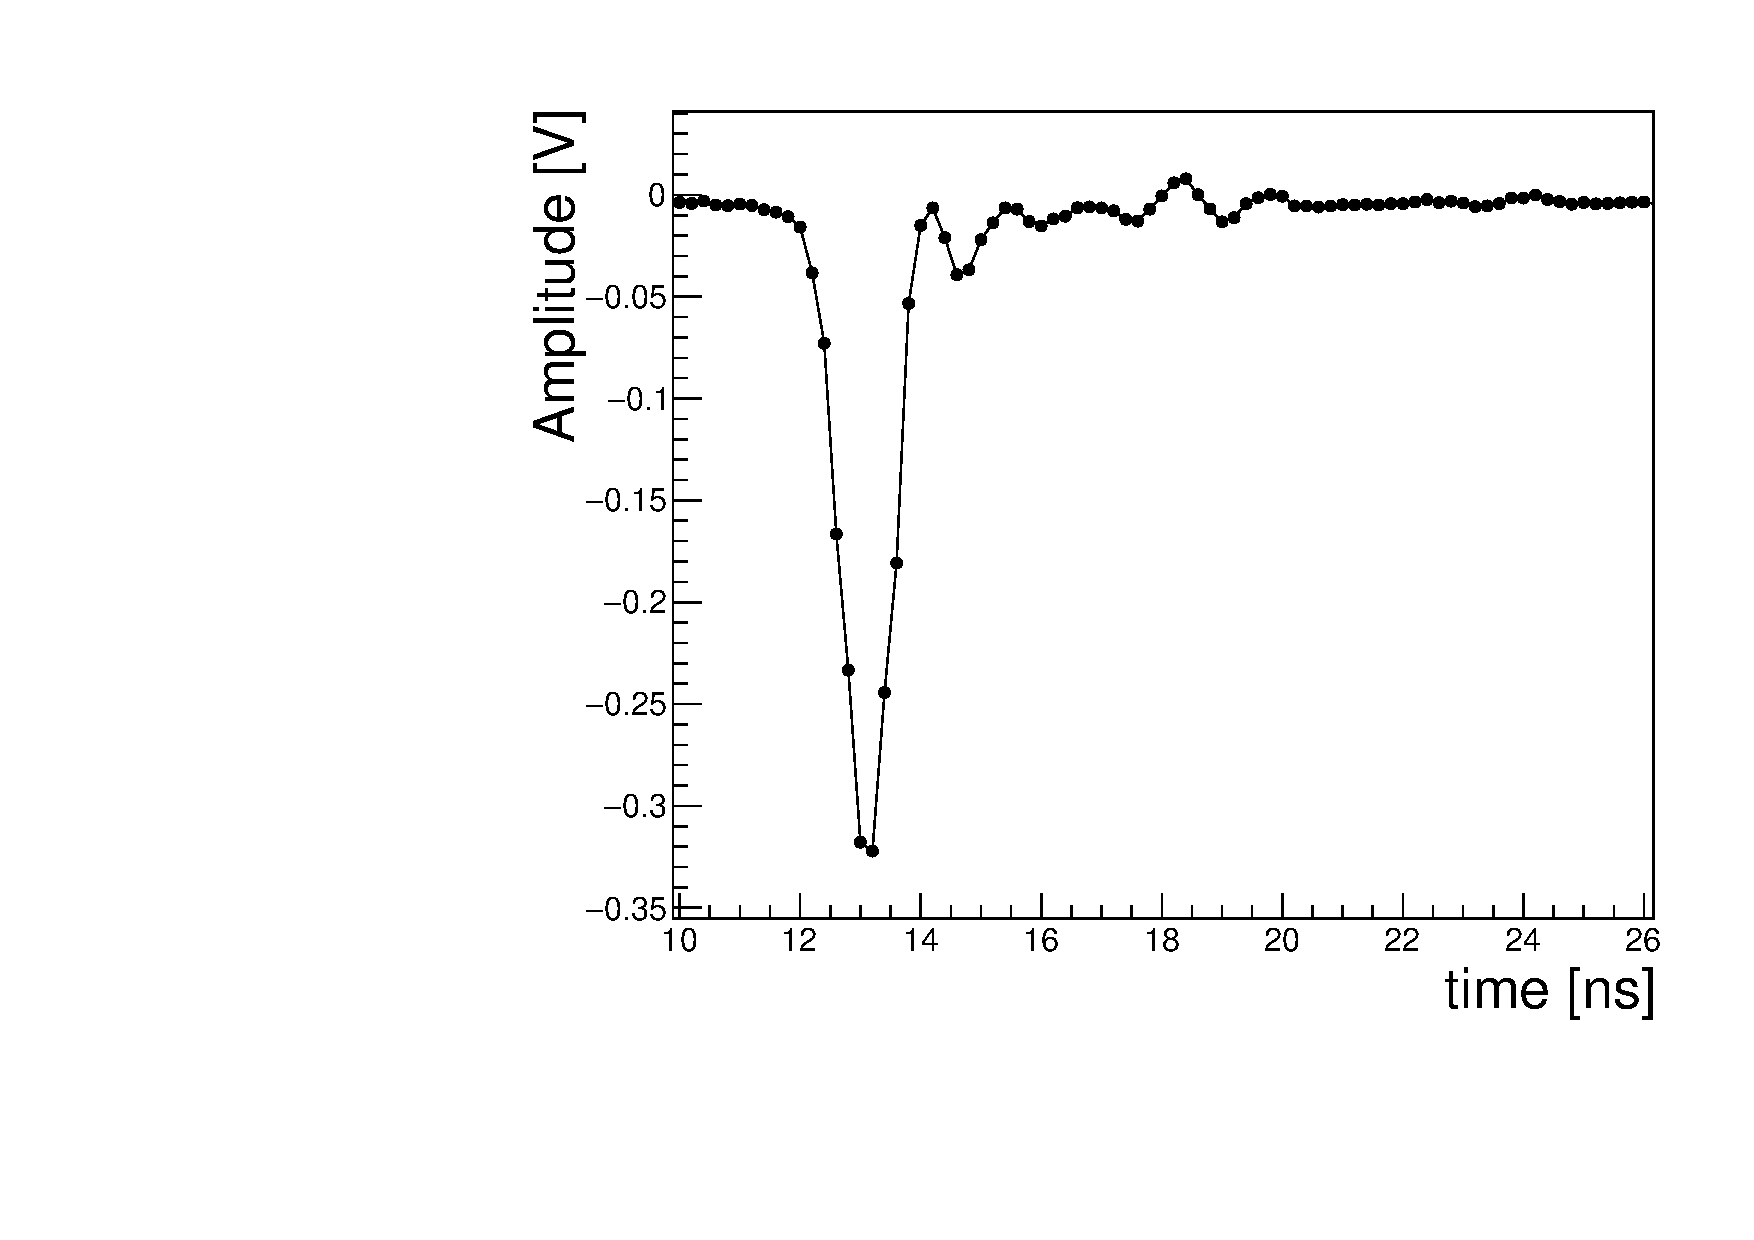
\includegraphics[width=8cm]{Images/expulse/pulsepix_30_2_12.pdf}
	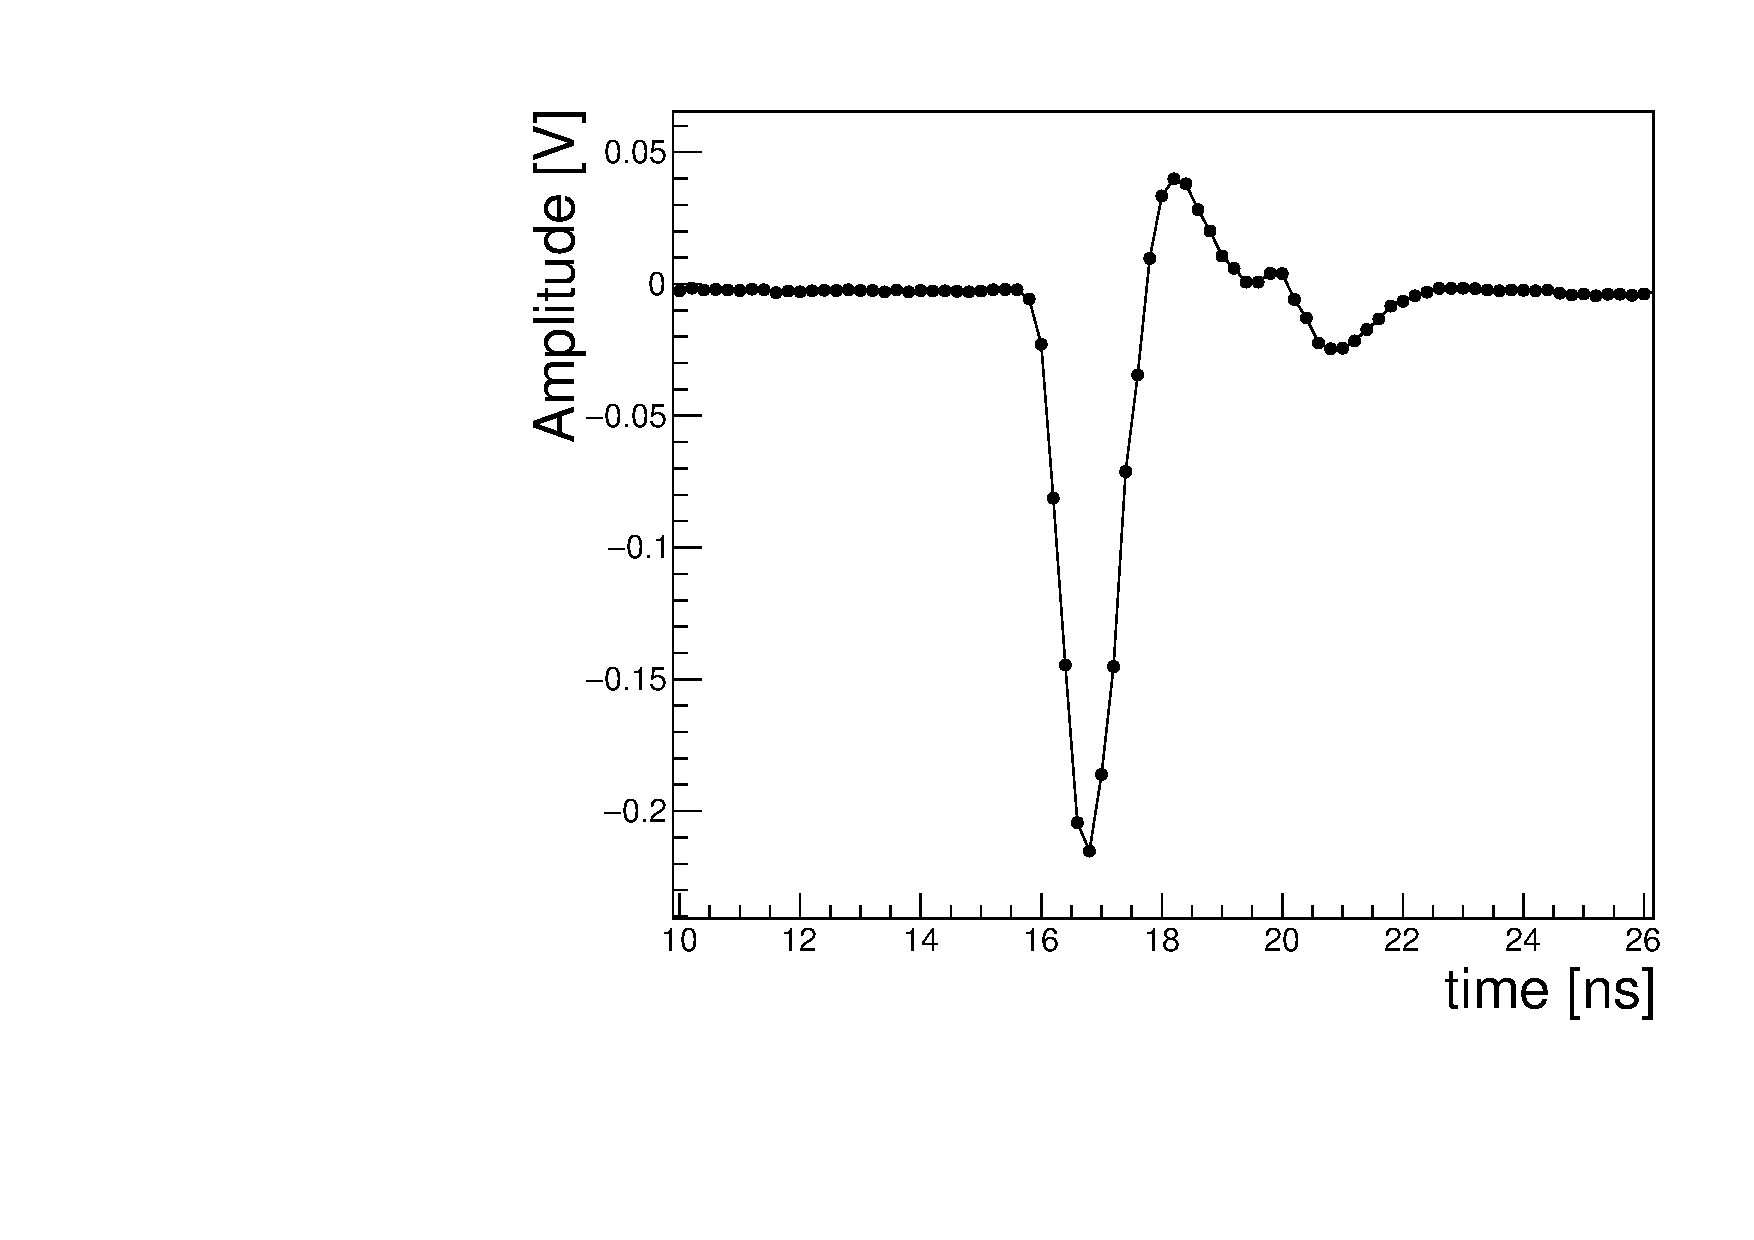
\includegraphics[width=8cm]{Images/expulse/pulseref_30_2_10.pdf}
	\caption{\small Example of a digitized signal from a single Photonis pixel (top) and Photek (bottom) MCP following a high-energy electron shower, via DRS4.}
	\label{fig:expulse}
\end{figure}



\title{\large}{\textbf{Experimental Setup}}

\begin{figure}[htbp]
	\centering
	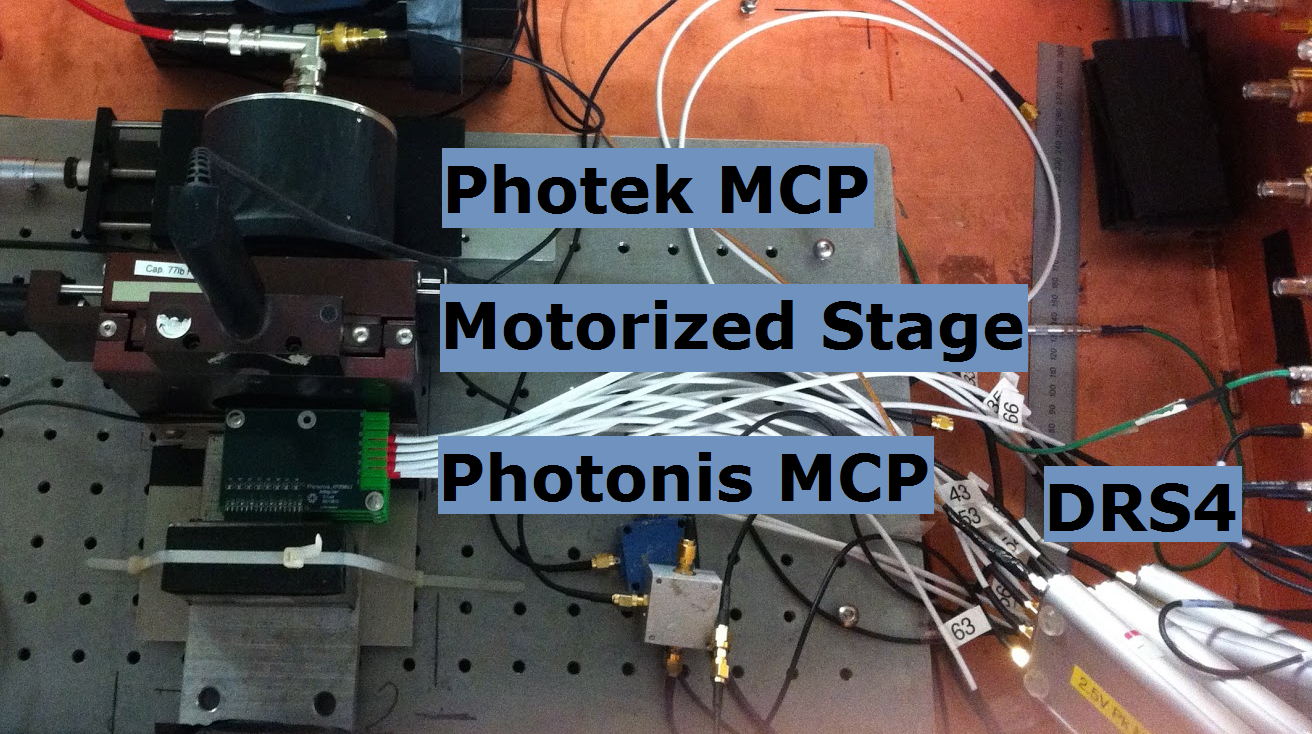
\includegraphics[width=8cm]{Images/setup/setup.png}
	\caption{\small Detector setup. Shown inside the dark box are the Photonis MCP on the motorized stage, the Photek MCP used as a reference time-stamp, and the DRS4 waveform digitizers.}
	\label{fig:setup}
\end{figure}

The Fermilab Test Beam Facility was used to obtain an \SI{8}{\giga\electronvolt} electron beam.
A differential Cherenkov counter was used to select for electron events.
All other detectors were located inside a dark box lined with copper foil for electromagnetic shielding.
A \SI{1.7}{\milli\meter}$\times$\SI{2.0}{\milli\meter} scintillation counter was used as a trigger.
A \SI{41}{\milli\meter\squared} aperture Photek 240, whose time resolution was previously measured as \SI{15}{\pico\second}, was used as a reference time-stamp for the incoming particles.
Nine channels of an eight-by-eight channel Photonis XP85011 MCP were used, set on a high precision motorized stage. One of the pixels was later realized to have been dead, reducing the count to eight channels.
A tungsten absorber of 3 times the radiation length (circa \SI{1}{\centi\meter}) was placed in front of this MCP.
Four DRS4 high speed waveform digitizers were used to acquire the signals from the Photek and Photonis channels as well as the Cherenkov trigger.

The motorized stage was used to perform scans in the Y direction, and move the particle shower center to different locations on the MCP. This allows us to calculate the spatial resolution of the setup. An image of the setup is shown in Figure \ref{fig:setup}.



\title{\large}{\textbf{Shower Maximum Mean Calculation}}

\begin{figure}[htbp]
	\centering
	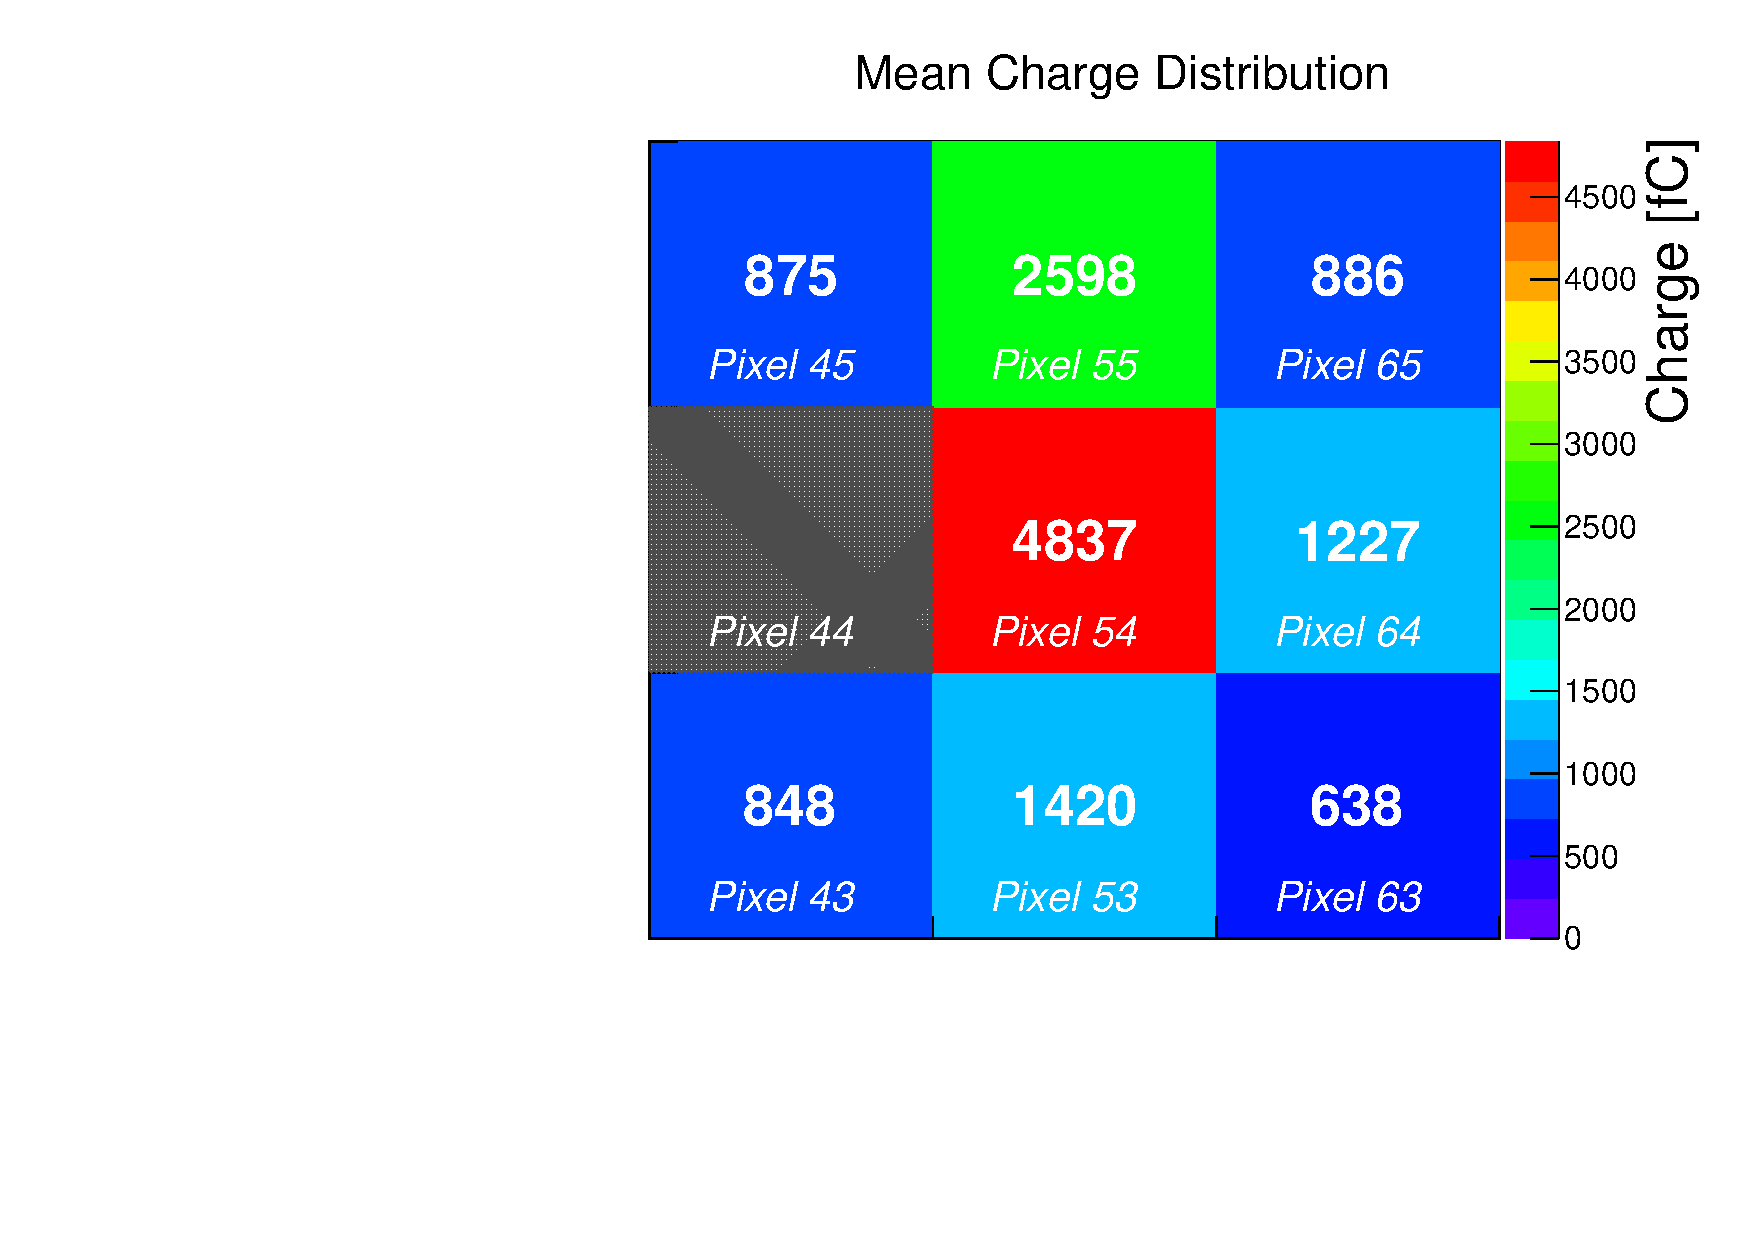
\includegraphics[width=8cm]{Images/exavint/exintrun30.pdf}
	\caption{\small Example of the average energy distribution on each pixel for a single run. Pixel 44 is dead. The charge distribution indicates that the shower maximum is located on the upper half of the center pixel.}
	\label{fig:exavint}
\end{figure}

\begin{figure*}[htbp]
	\centering
	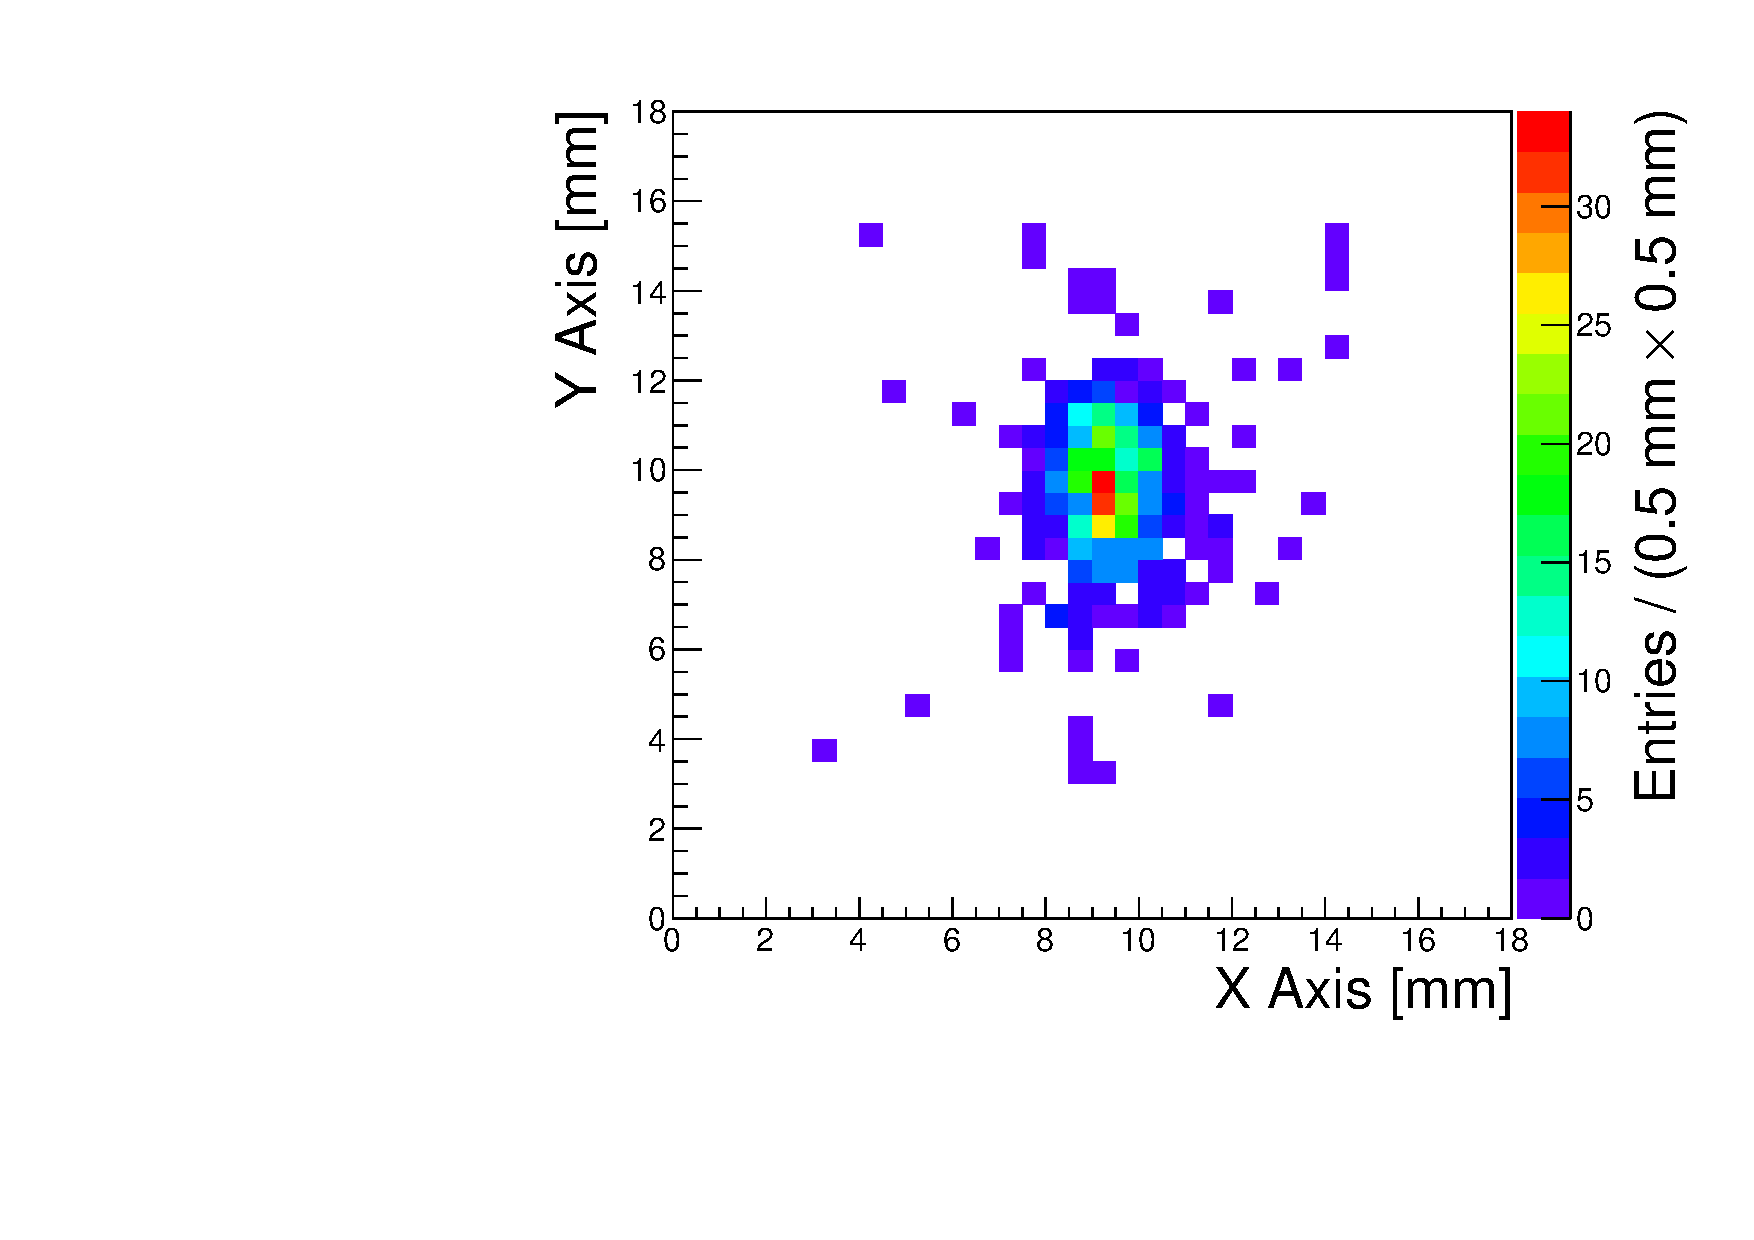
\includegraphics[width=8cm]{Images/centers/run30dist.pdf}
	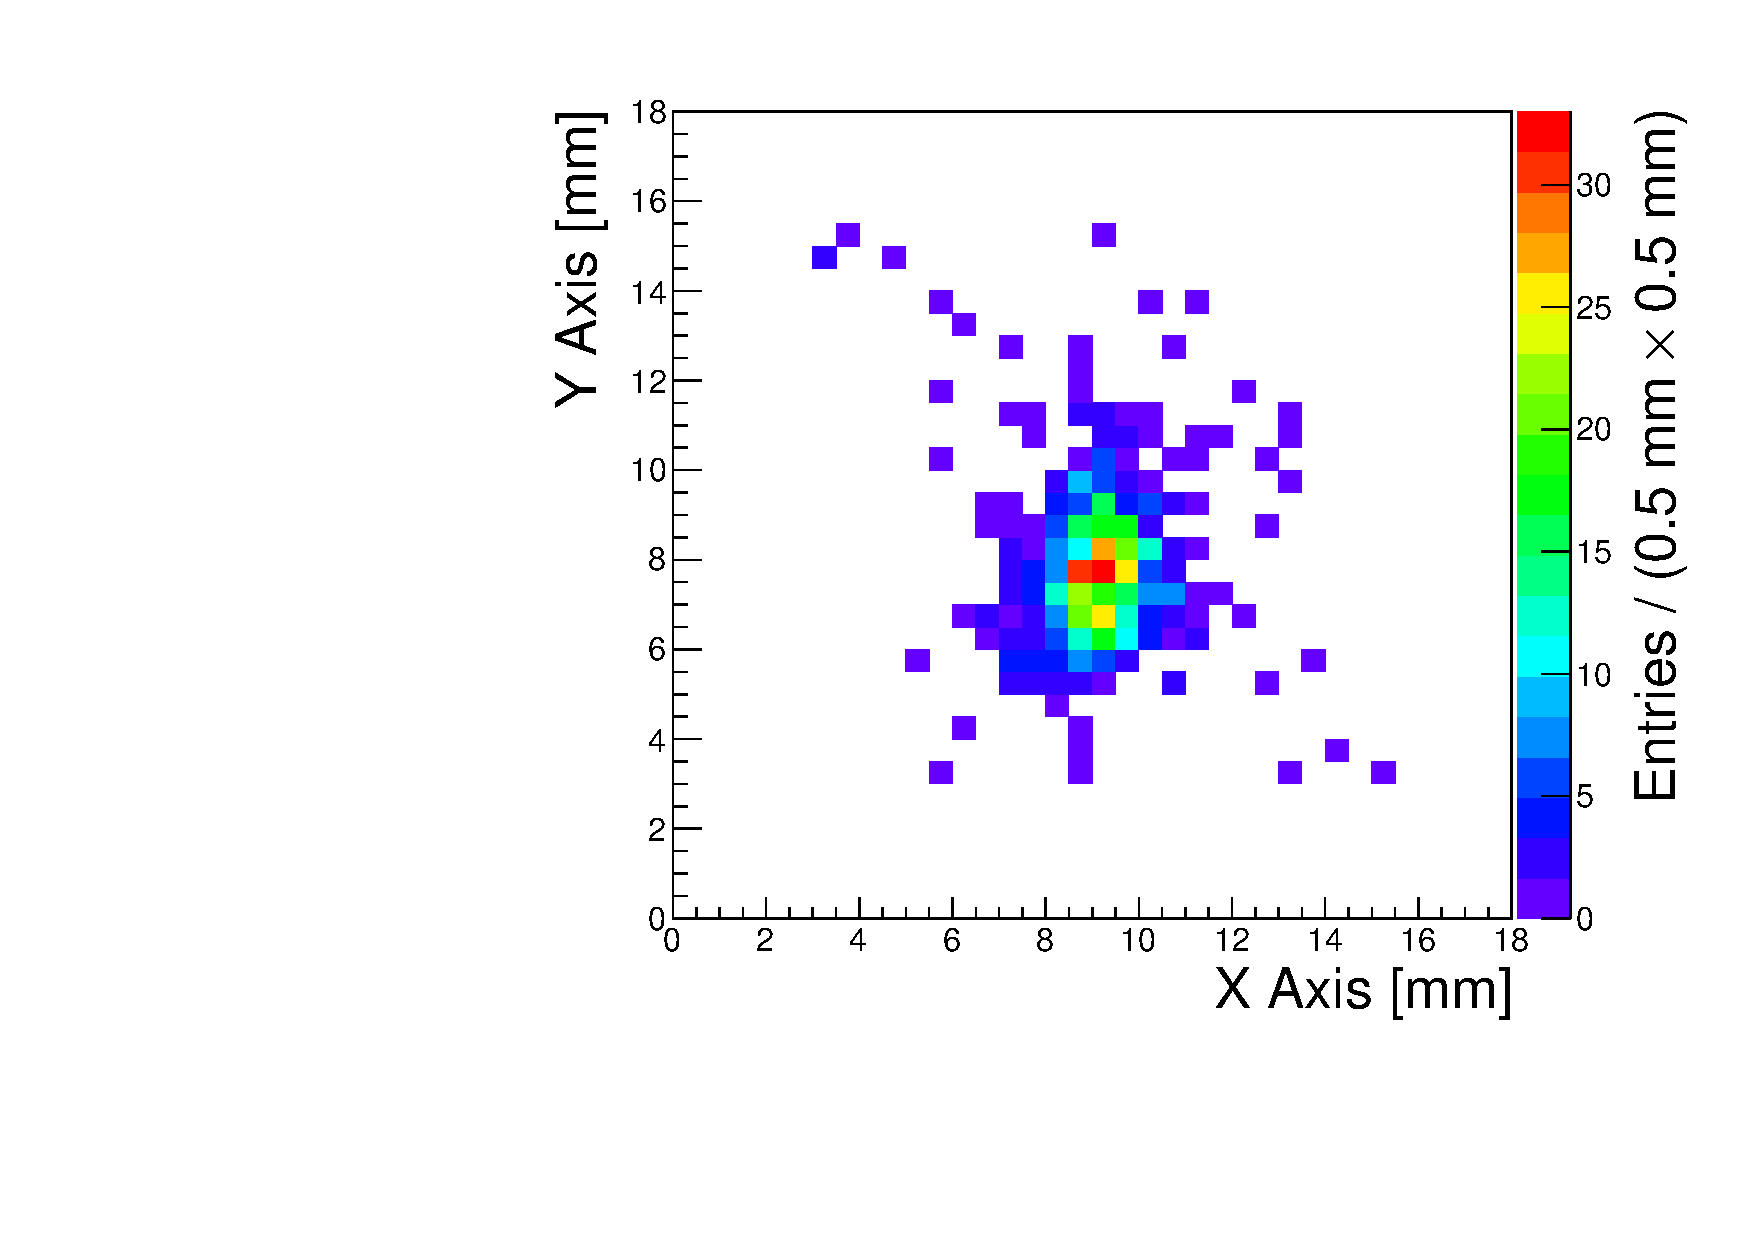
\includegraphics[width=8cm]{Images/centers/run32dist.pdf}
	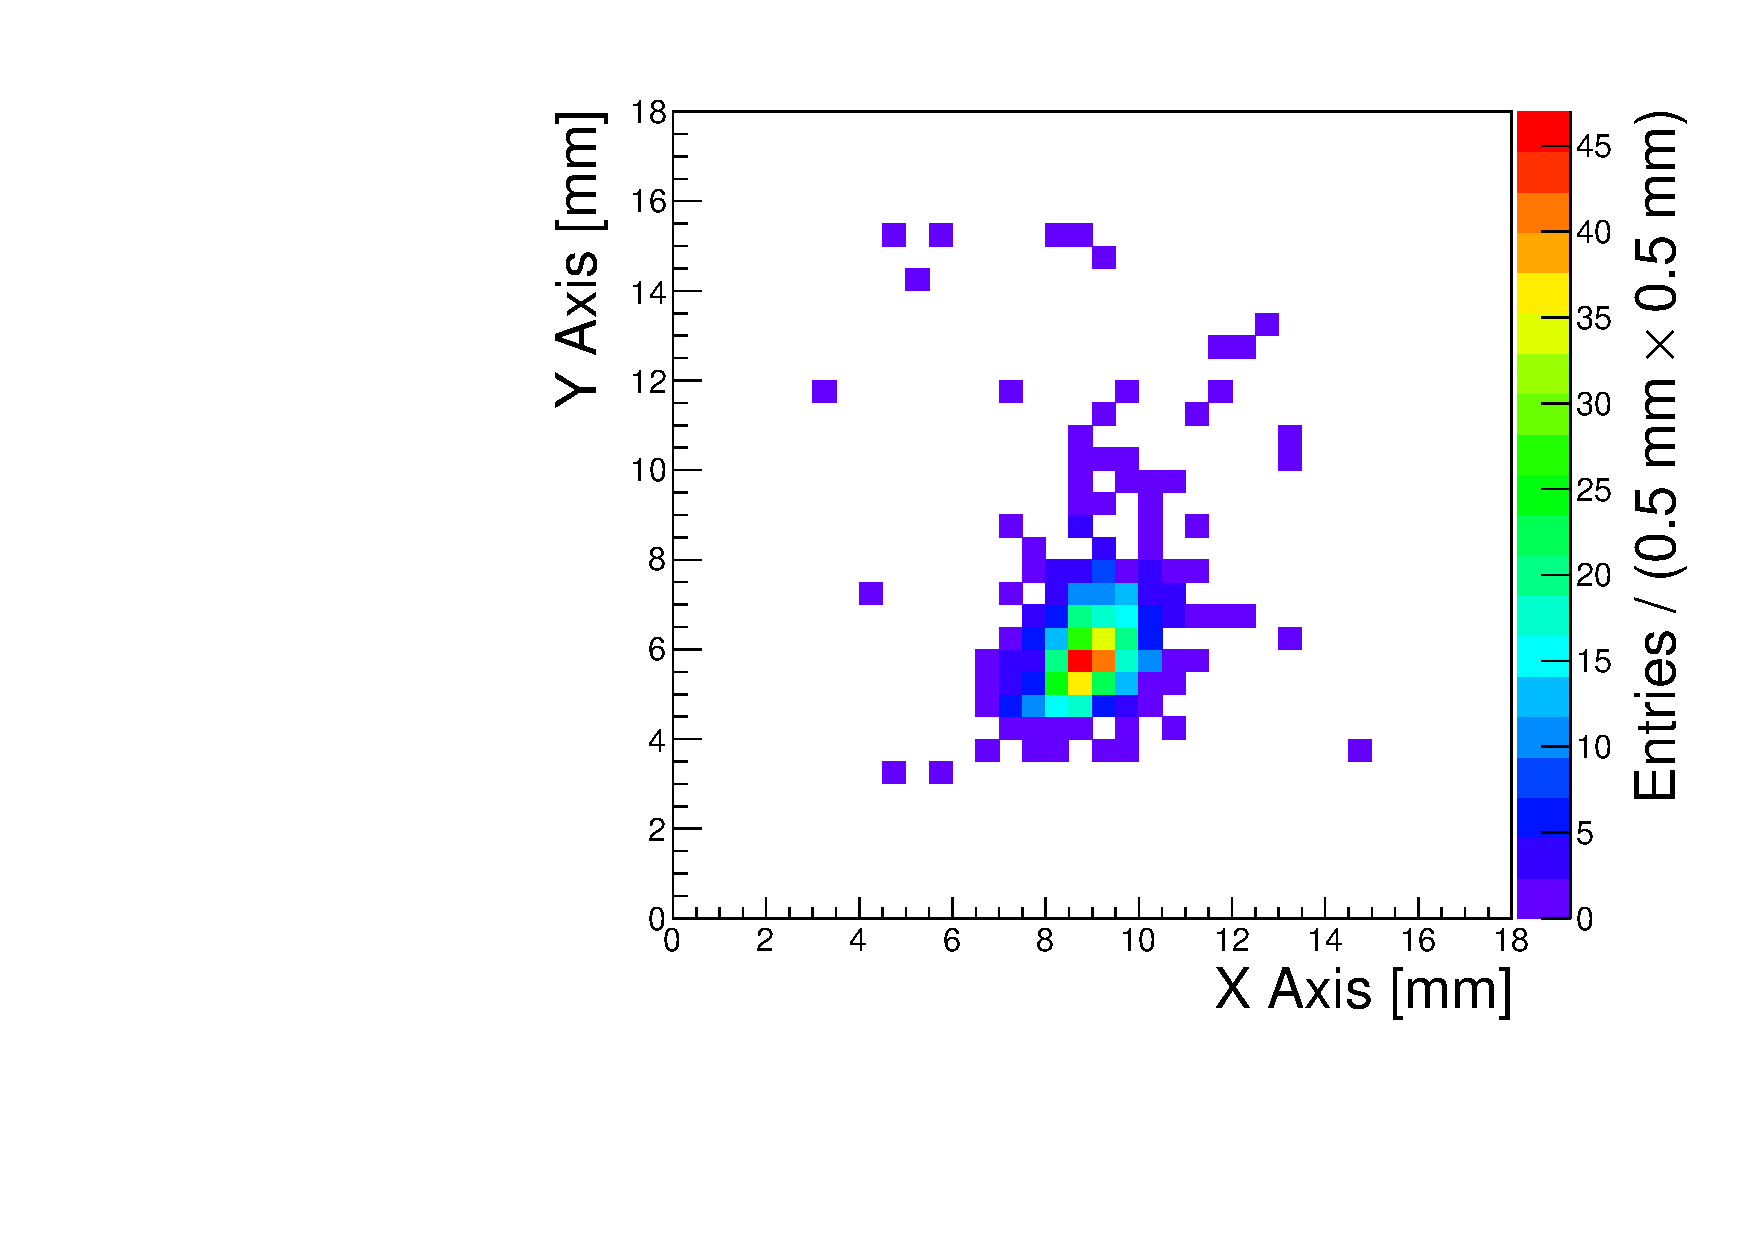
\includegraphics[width=8cm]{Images/centers/run34dist.pdf}
	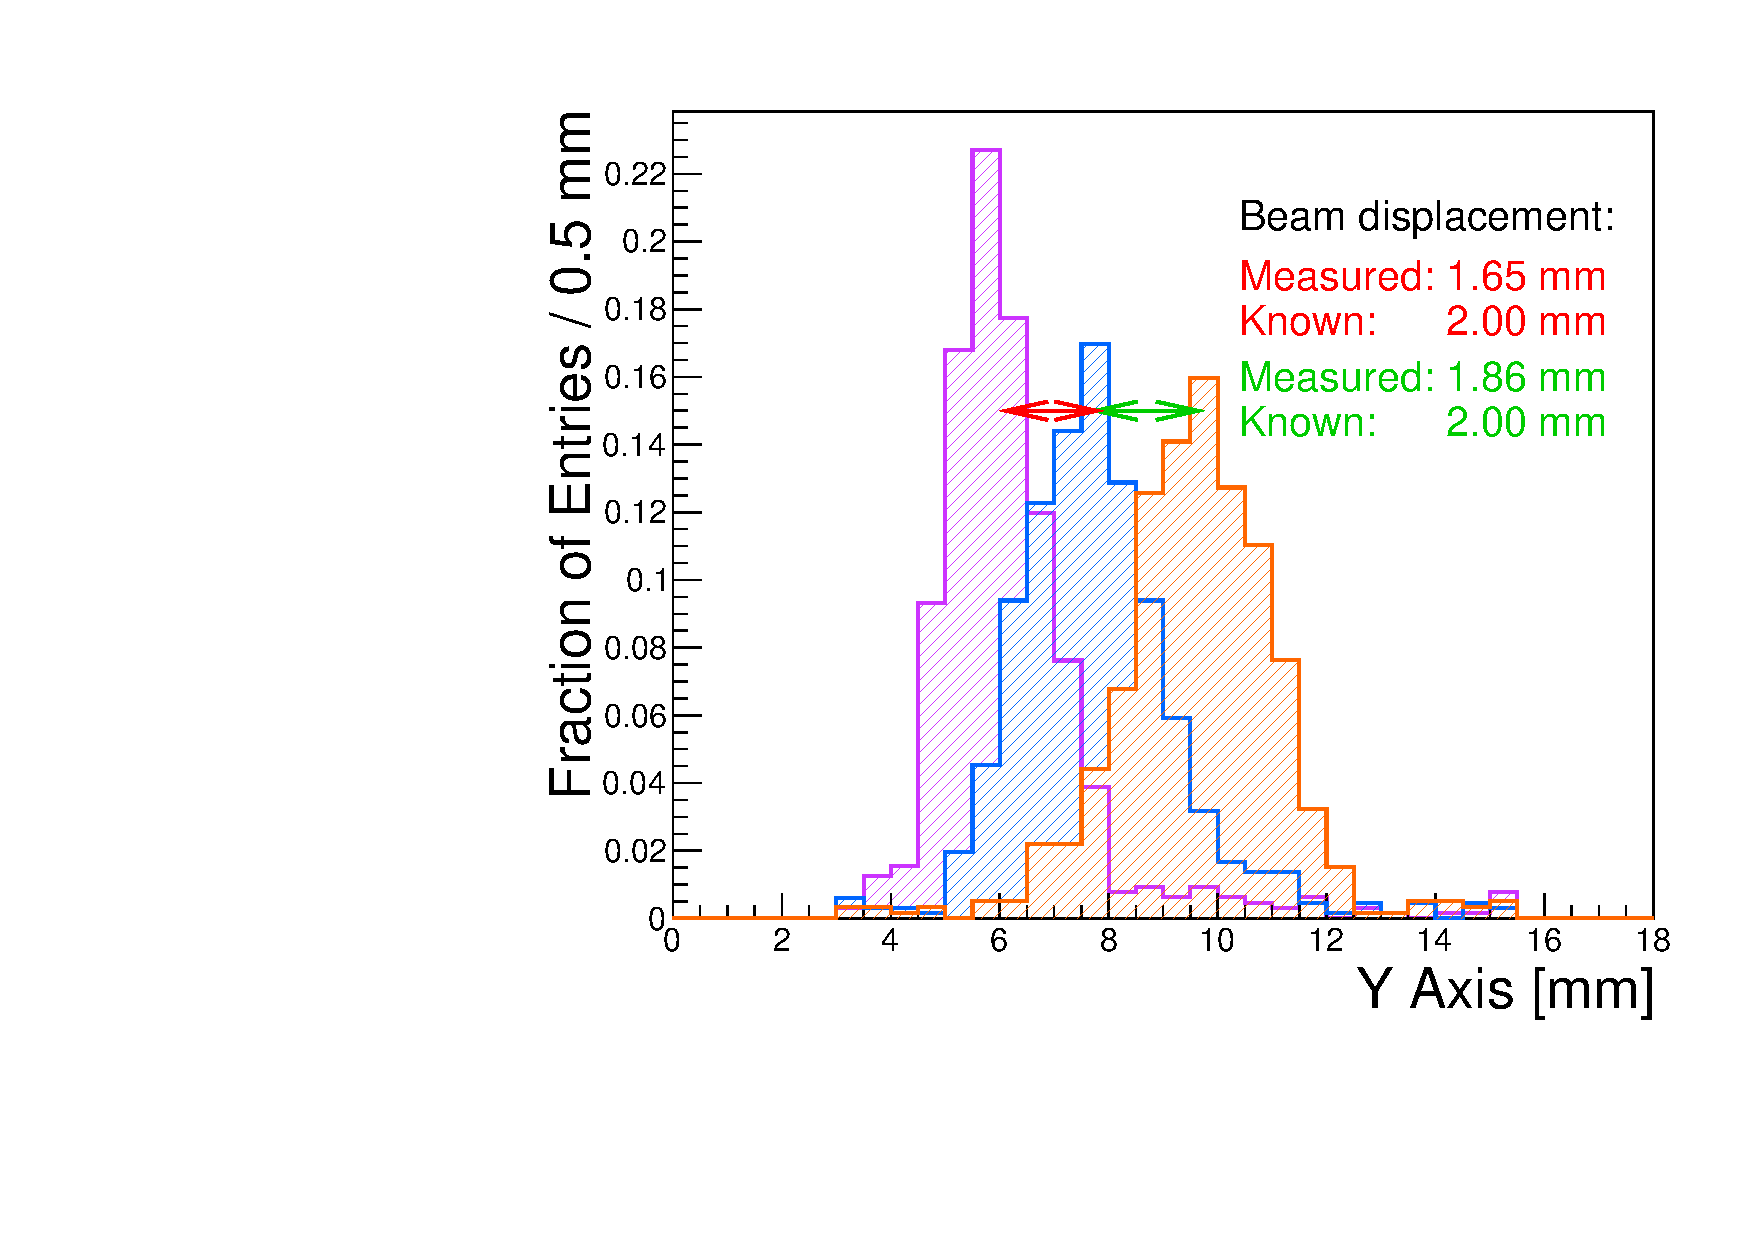
\includegraphics[width=8cm]{Images/centers/superimposed.pdf}
	\caption{\small Example of three shower-beam center distributions located at the bottom, center, and top of the MCP, calculated as described in the text. The last plot shows a projection onto the Y axis of all three distributions and their known and calculated maxima displacements.}
	\label{fig:centers}
\end{figure*}

A shower center can be calculated for each electron event by considering the strength of the signal at each pixel and finding the position via a weighted mean. As can be seen in Figure \ref{fig:exavint}, there is variation in the charge deposited in each pixel, which depends on the shower maximum.

The pixel size of the Photonis device is \SI{6}{\milli\meter}$\times$\SI{6}{\milli\meter}. Doing such a calculation allows us to obtain a shower-center position more precise than the pixel size.

The procedure for evaluating the strength of a signal involves integrating the signal pulse near the peak, effectively calculating the charge deposited onto the MCP. Specifically, we summed a total of nine sampled points centered around the highest one (subtracting DC offset). This effectively integrates the signal over \SI{1.6}{\nano\second}.

Finding the shower maximum by weighted average involves summing the center position of each pixel scaled by its signal strength, and dividing by the sum of all the signal strength values. Where $c_x,c_y$ are the components of the center of a pixel as measured from the bottom left corner of the array of active pixels, and $I$ is the scale factor (derived from the signal integral):
\[
\vec{\mathbf{{\mu}}} =
\frac{\sum_{i\in\text{pixels}} Q_i \vec{c}_i}
{\sum_{i\in\text{pixels}} Q_i}
\]
%\left(\begin{matrix}c_x\\c_y\end{matrix}\right)

As can be seen in Figure \ref{fig:centers}, the shower-center roughly follows a 2 dimensional normal distribution. Thus, fitting a 2D Gaussian function allows us to find the mean of the distribution.

\title{\large}{\textbf{Spatial Resolution}}

\begin{figure}[htbp]
	\centering
	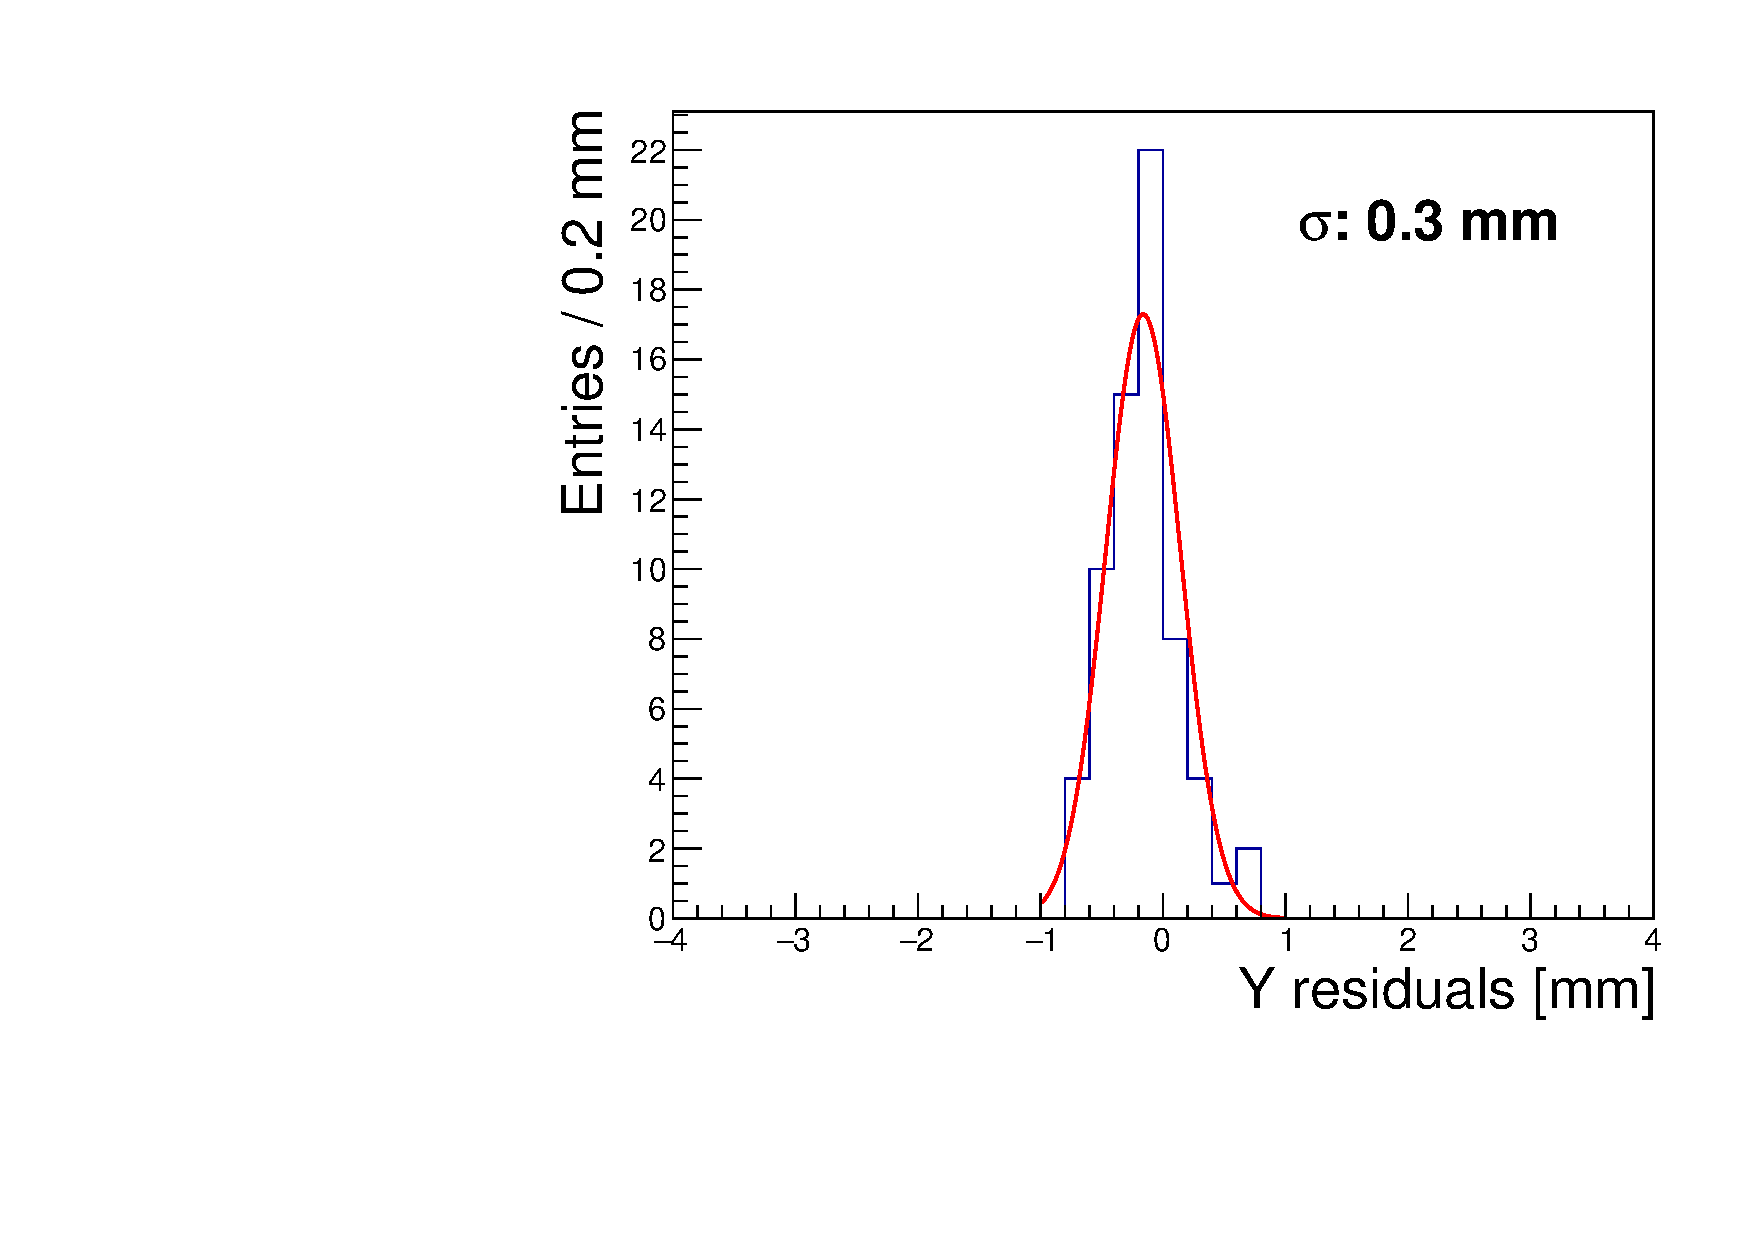
\includegraphics[width=8cm]{Images/sres/sres_cutoff.pdf}
	\caption{\small The spatial resolution in the Y direction. The resolution is about \SI{0.3}{\milli\meter}, much smaller than the \SI{6}{\milli\meter} pixel size of the MCP.}
	\label{fig:sres}
\end{figure}

The data set of shower maxima obtained can be used to find the spatial resolution, by comparing these measured displacements between runs to the known displacements, which are the amount we moved the MCP's stage. The spatial resolution is defined as the standard deviation of the error: $(y_\text{measured}-y_\text{measured}') - \Delta y_\text{known}$. As seen in Figure \ref{fig:sres}, the resolution obtained is \SI{0.8}{\milli\meter}.



\title{\large}{\textbf{Time Resolution and Weighted Time Stamp}}

A set of quality criteria was used with the goal to eliminate abnormal pulses from the readout that would affect the calculations and fits for determining the time-stamp.

The time resolution is found by subtracting the reference channel's time-stamp from the single-pixel channel time-stamp. These time-stamps are defined as the peak of the signal pulse. The signal signed is flipped and the time-stamp is obtained by using the mean of a Gaussian fit in the neighborhood of the peak (see \ref{fig:expulse}. The time resolution is the standard deviation of the time difference of these time-stamps.

The time resolution at an individual pixel level varies from run to run, and depends on its vicinity to the center of the beam and the signal strength of its pulses.

\begin{figure}[htbp]
	\centering
	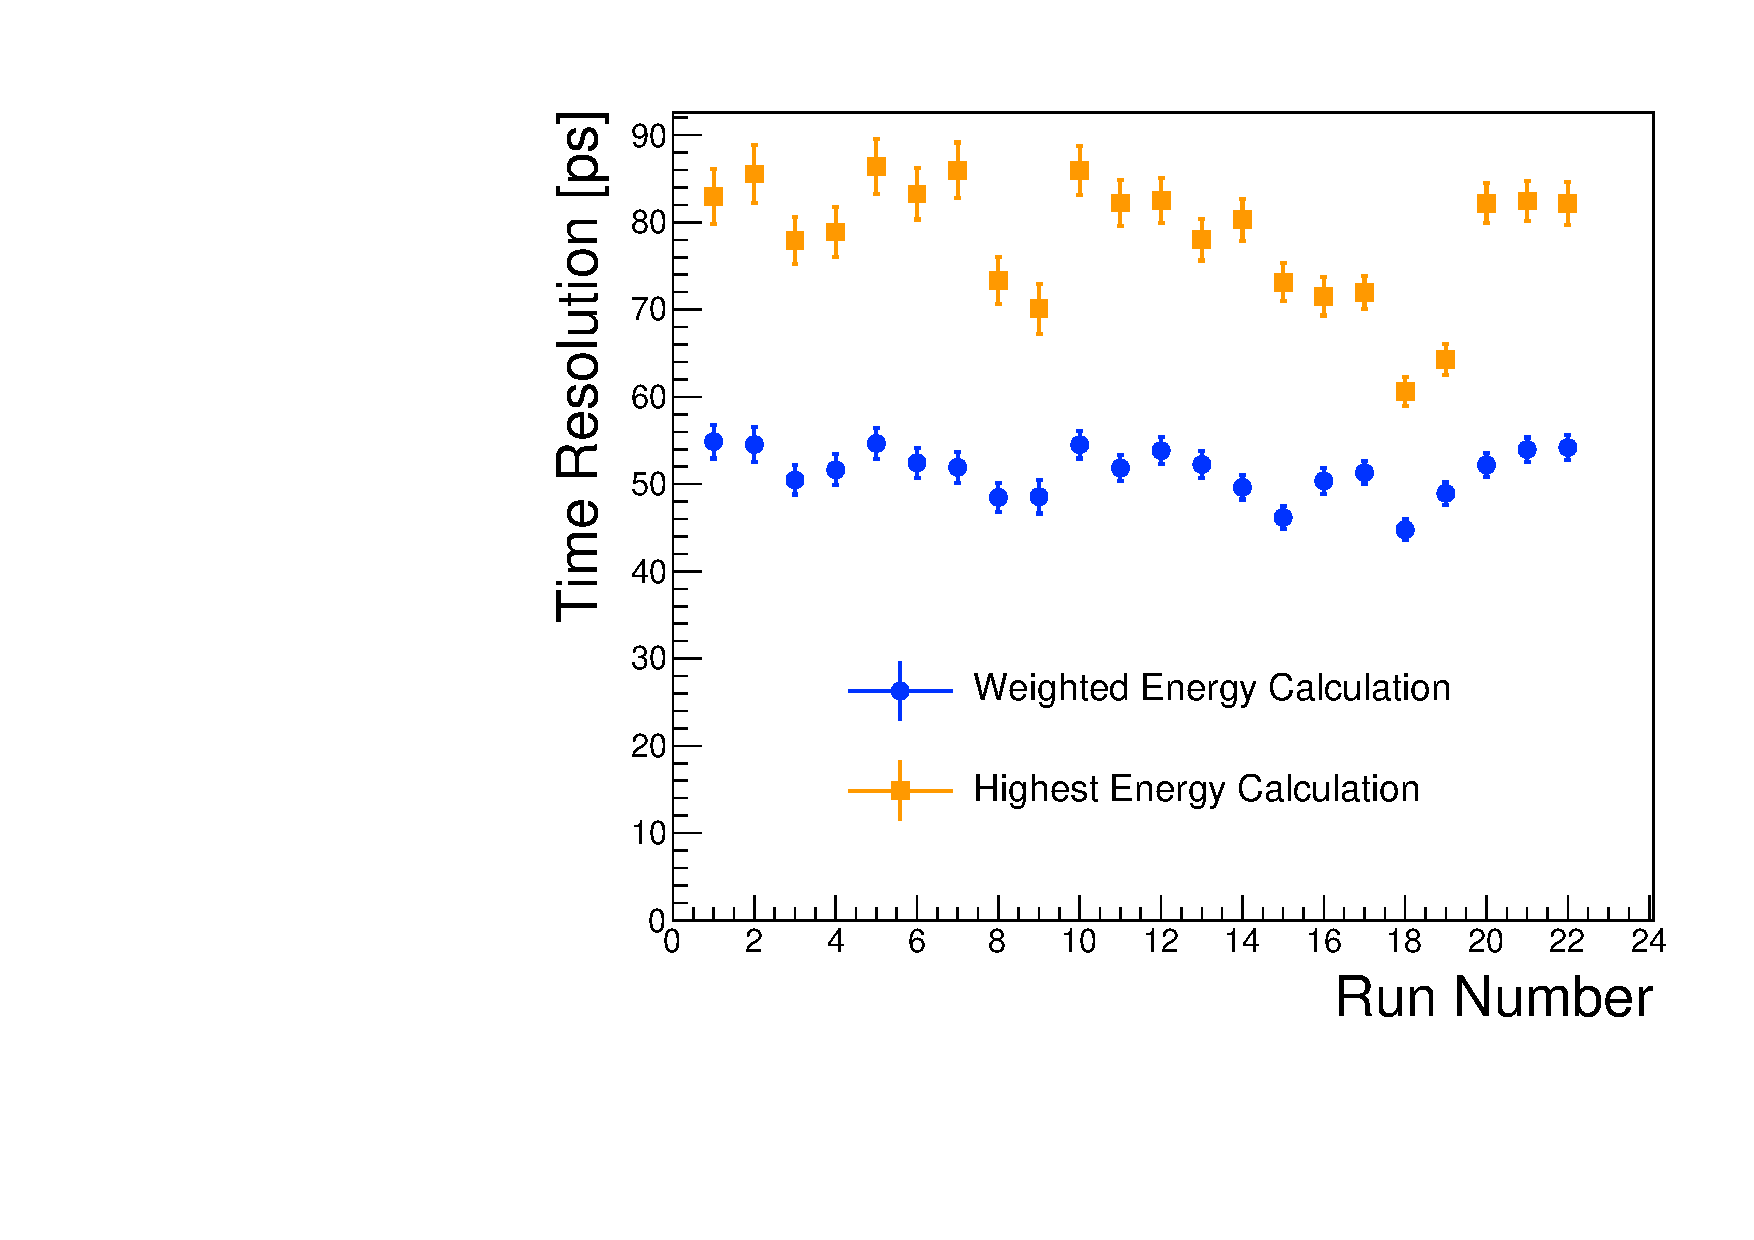
\includegraphics[width=8cm]{Images/wtres/tresperrun.pdf}
	\caption{\small Time resolution found for each run. The time-stamp weighting method consistently results in under \SI{60}{\pico\second}. Notice how the highest-signal-pixel method for picking the time-stamp value is significantly worse.}
	\label{fig:wtres}
\end{figure}

However, it was found that the time resolution of the system could be calculated by a similar weighting method as used to find the shower maxima. The reasoning behind this is that higher amplitude signals generally have better time resolution (due to sharper peaks). The time-stamps are averaged by weighting a pixel's time-stamp with either the signal integral.
\[\bar{\Delta t} =
\frac{\sum_{i\in\text{pixels}} Q_i \Delta t_i}
{\sum_{i\in\text{pixels}} Q_i}
\]
This method generally improves on the best time-resolution pixel for a run, and results in a consistent time resolution of less than \SI{60}{\pico\second}, and as low as \SI{45}{\pico\second} (see Figure \ref{fig:wtres}). Note that this method worked better than picking the time-stamp associated with the highest amplitude signal for a given event. This is because the time resolution in this latter method approaches that of the pixel closest to the shower maximum. Taking into consideration the whole active MCP board increases the accuracy.

\begin{figure}[htbp]
	\centering
	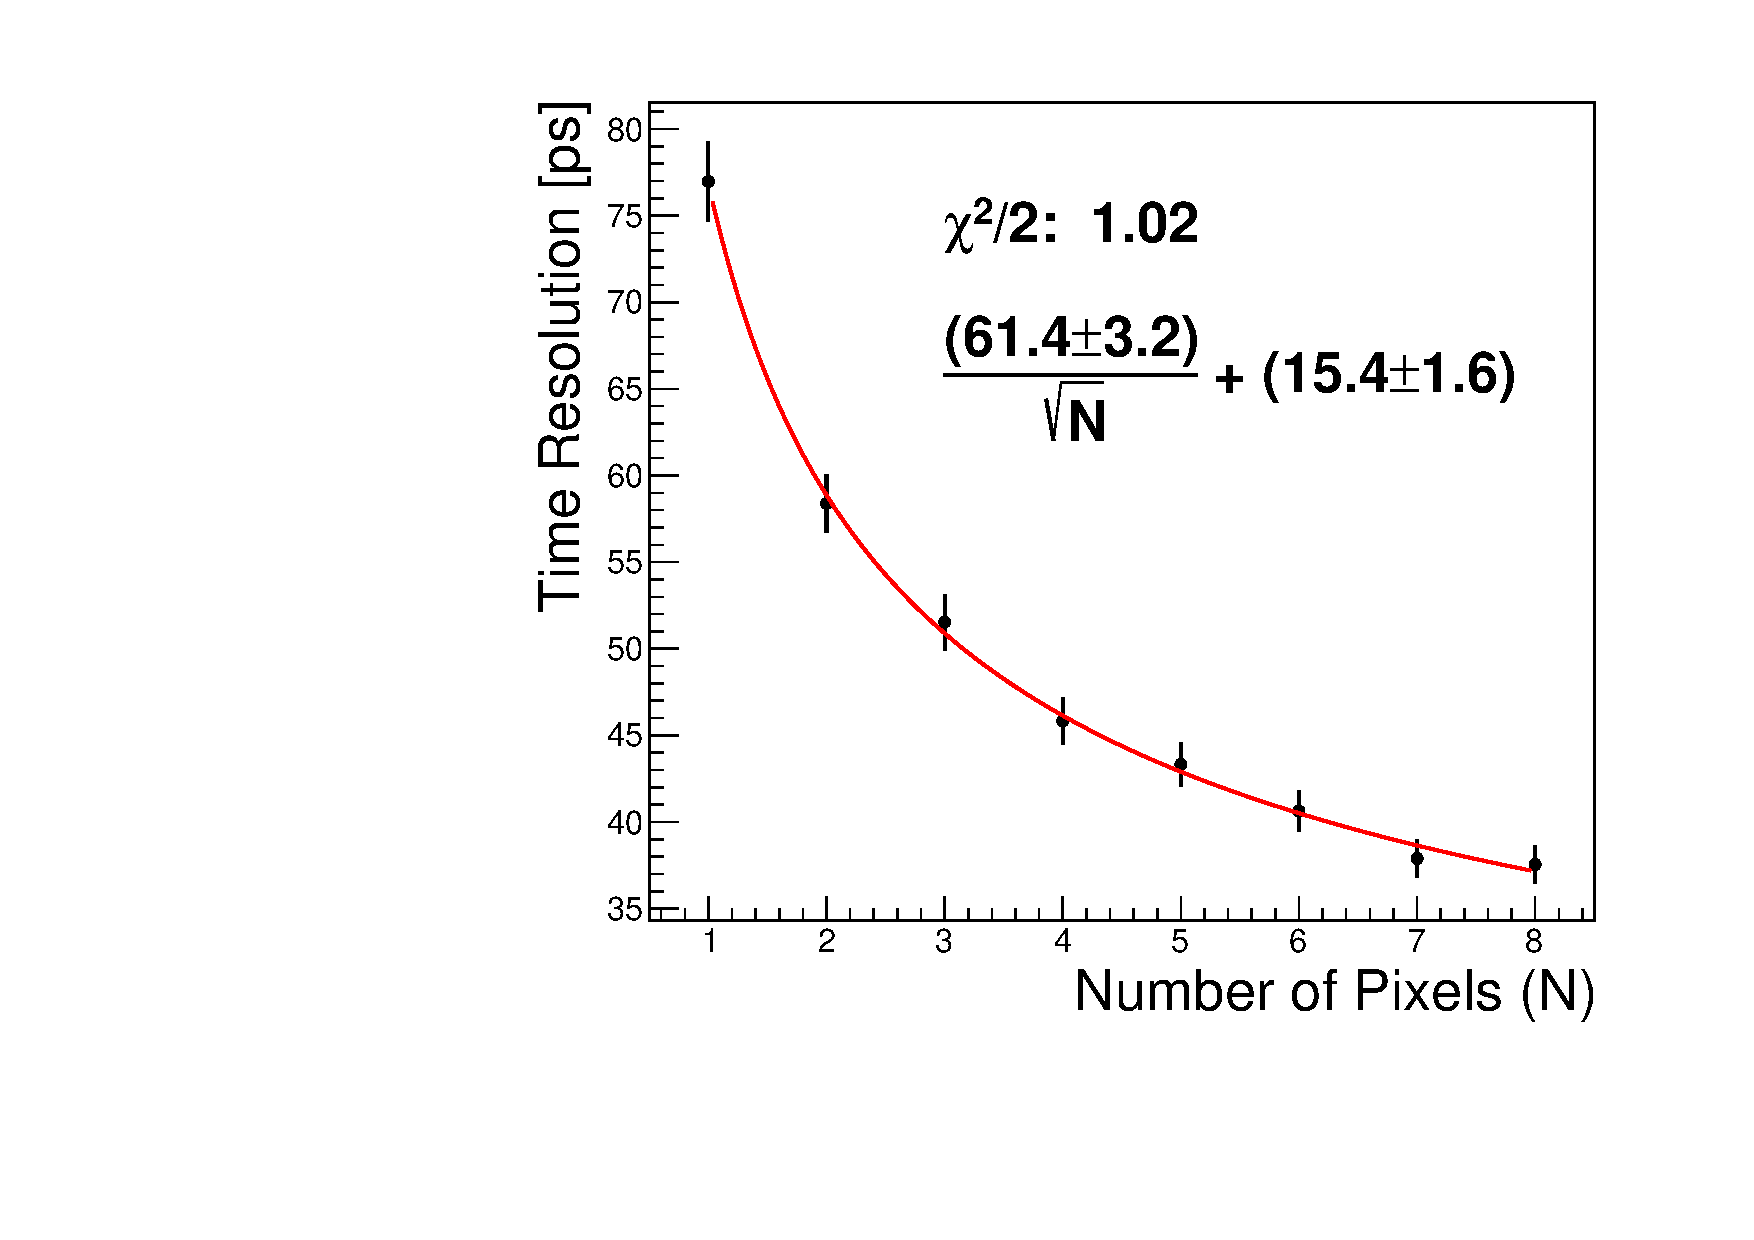
\includegraphics[width=8cm]{Images/sqrtN/t1065_run_38_Dt_IWP.pdf}
	\caption{\small Generally the time resolution appears to scale by a factor of $1/\sqrt{N}$, the number of pixels used to average the time stamp.}
	\label{fig:sqrtN}
\end{figure}

Figure \ref{sqrtN} demonstrates the increasing timing performance with increasing number of pixels from a single run. Generally the time resolution value decreases by the square root of the number of pixels.


\title{\large}{\textbf{Calibrated Time Resolution}}

\begin{figure*}[htbp]
	\centering
	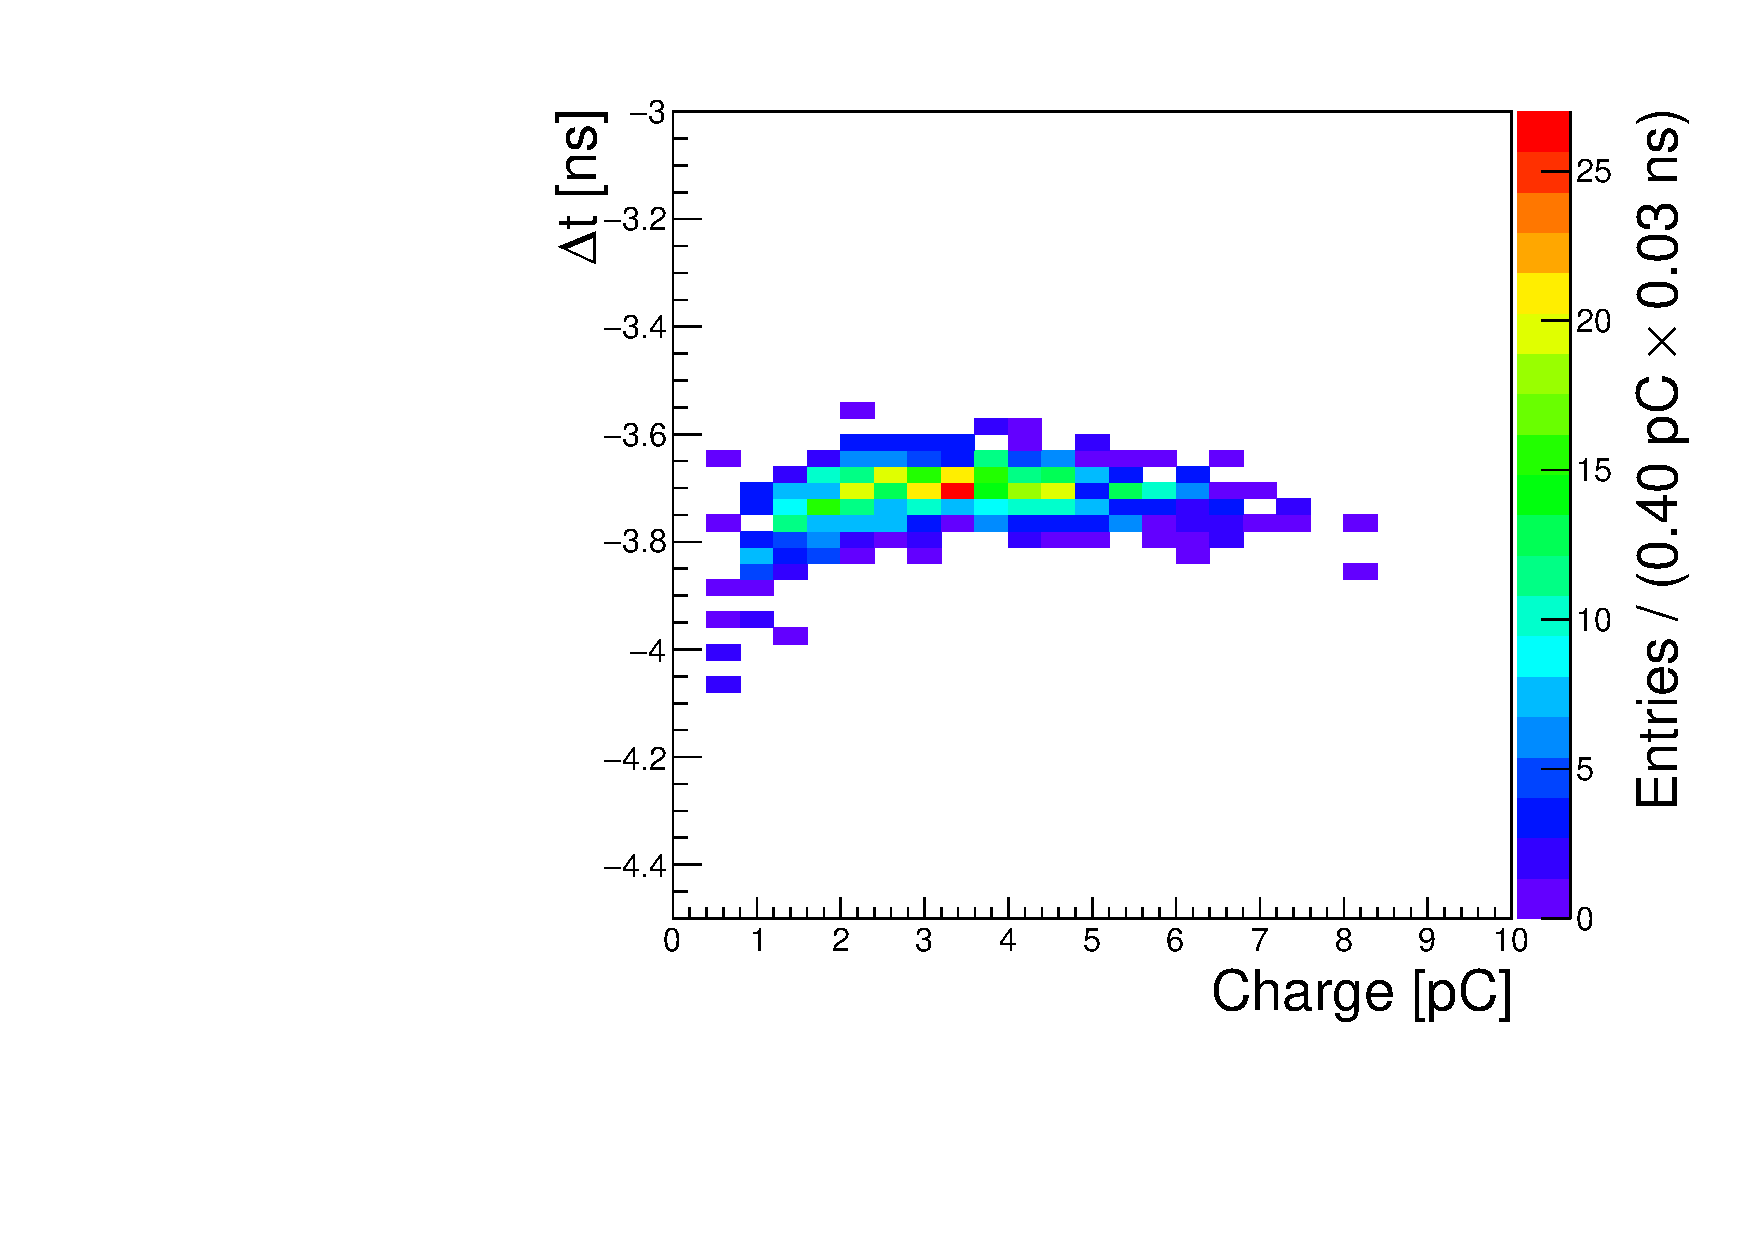
\includegraphics[width=8cm]{Images/dt-int/dtint30_o22.pdf}
	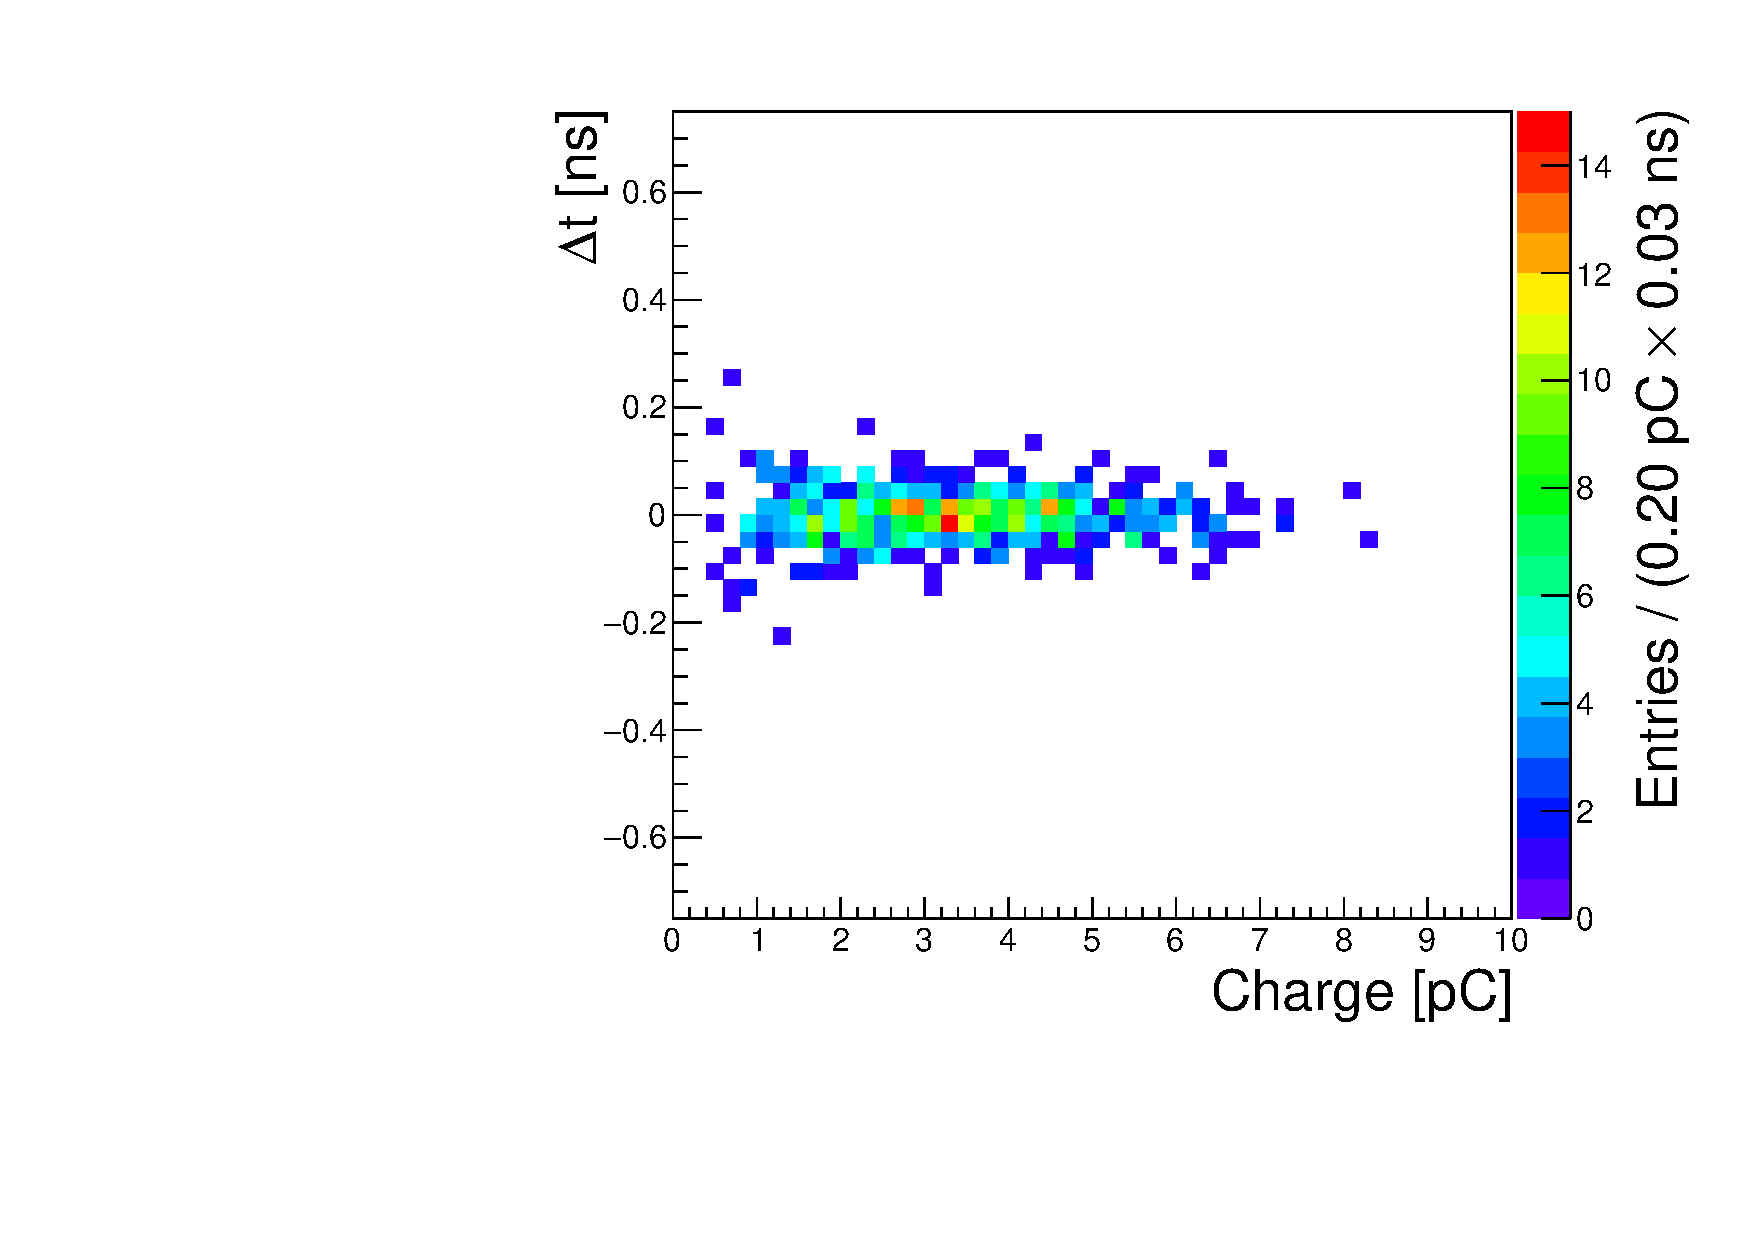
\includegraphics[width=8cm]{Images/dt-int/dtint30_c22.pdf}
	\caption{\small Left: characteristic distribution of $\Delta t$ with respect to the signal's integral. Notice that the relation is not constant. The $\Delta t$ value can be calibrated in order to obtain such a constant relation. Right: the same distribution after self-correction. Coarser bins are used for calibration to guarantee more events.}
	\label{fig:dt-int}
\end{figure*}

It was also found, as shown in Figure \ref{fig:dt-int}, that the time-stamp to signal integral is not a constant relation. This means that in principle a calibration is possible to obtain a superior time resolution.

\begin{figure}[htbp]
	\centering
	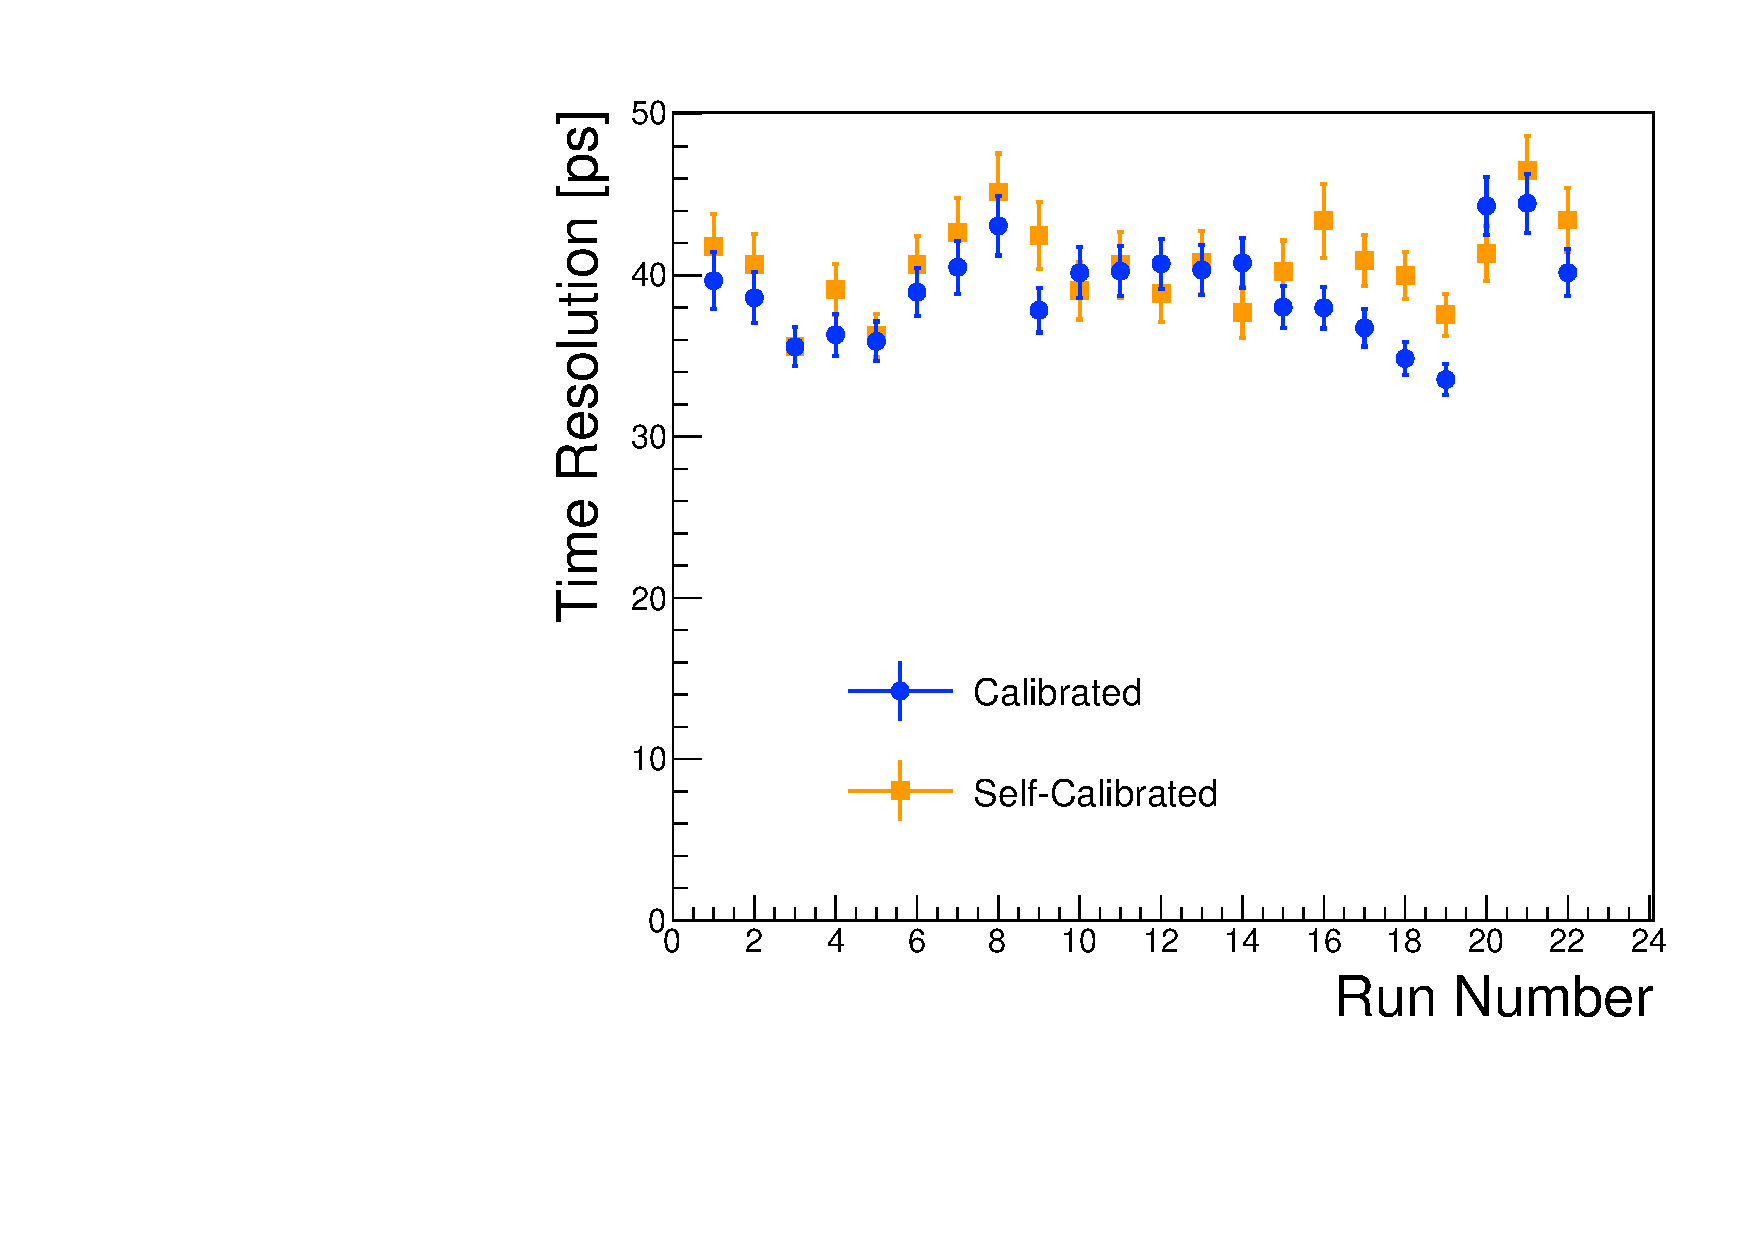
\includegraphics[width=8cm]{Images/calibtres/timerescalib.pdf}
	\caption{\small This plot includes the time resolution for each run after applying correction factors found using run 3, and the time resolution obtained from calibrating a run against itself. The improvement from no calibration is important. Notice how the globally calibrated time resolution values do not differ significantly from the self-calibration time resolutions.}
	\label{fig:calib}
\end{figure}

This calibration performed is piecewise and works as follows. The time-integral function is split into slices. The mean is found for each slice and used to recenter the distribution around 0.

One run was chosen as a calibration run, and the values used to correct all other runs. The issue with this is that when the shower maximum is located at different positions for the different runs, the dynamic range of pixels changes, introducing error to the value of the corrections for some slices. Nonetheless, this calibration improves the time resolution by about \SI{10}{\pico\second}, as shown in Figure \ref{fig:calib}; the time resolutions where found to be in the range 35-\SI{45}{\pico\second}.

\begin{figure*}[htbp]
	\centering
	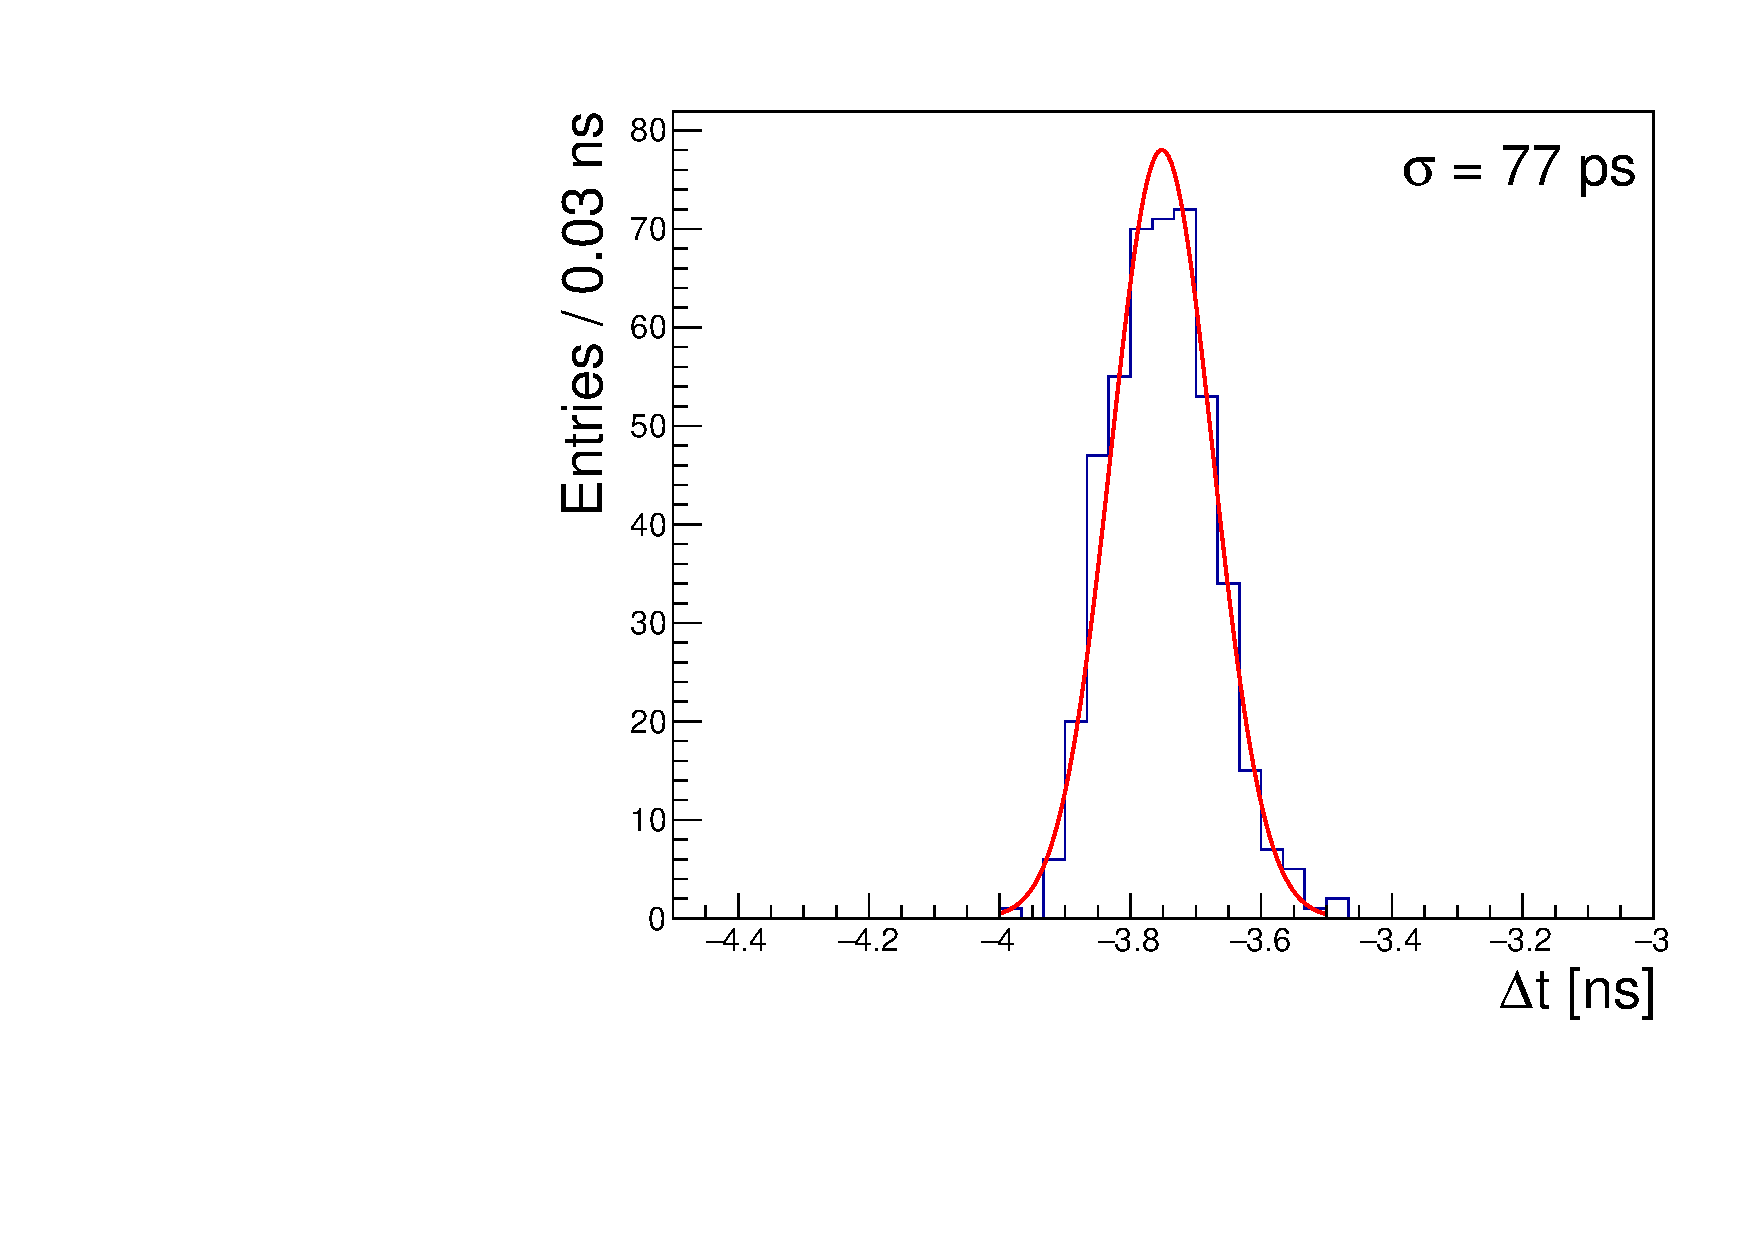
\includegraphics[width=8cm]{Images/exdt/exdtHI.pdf}
	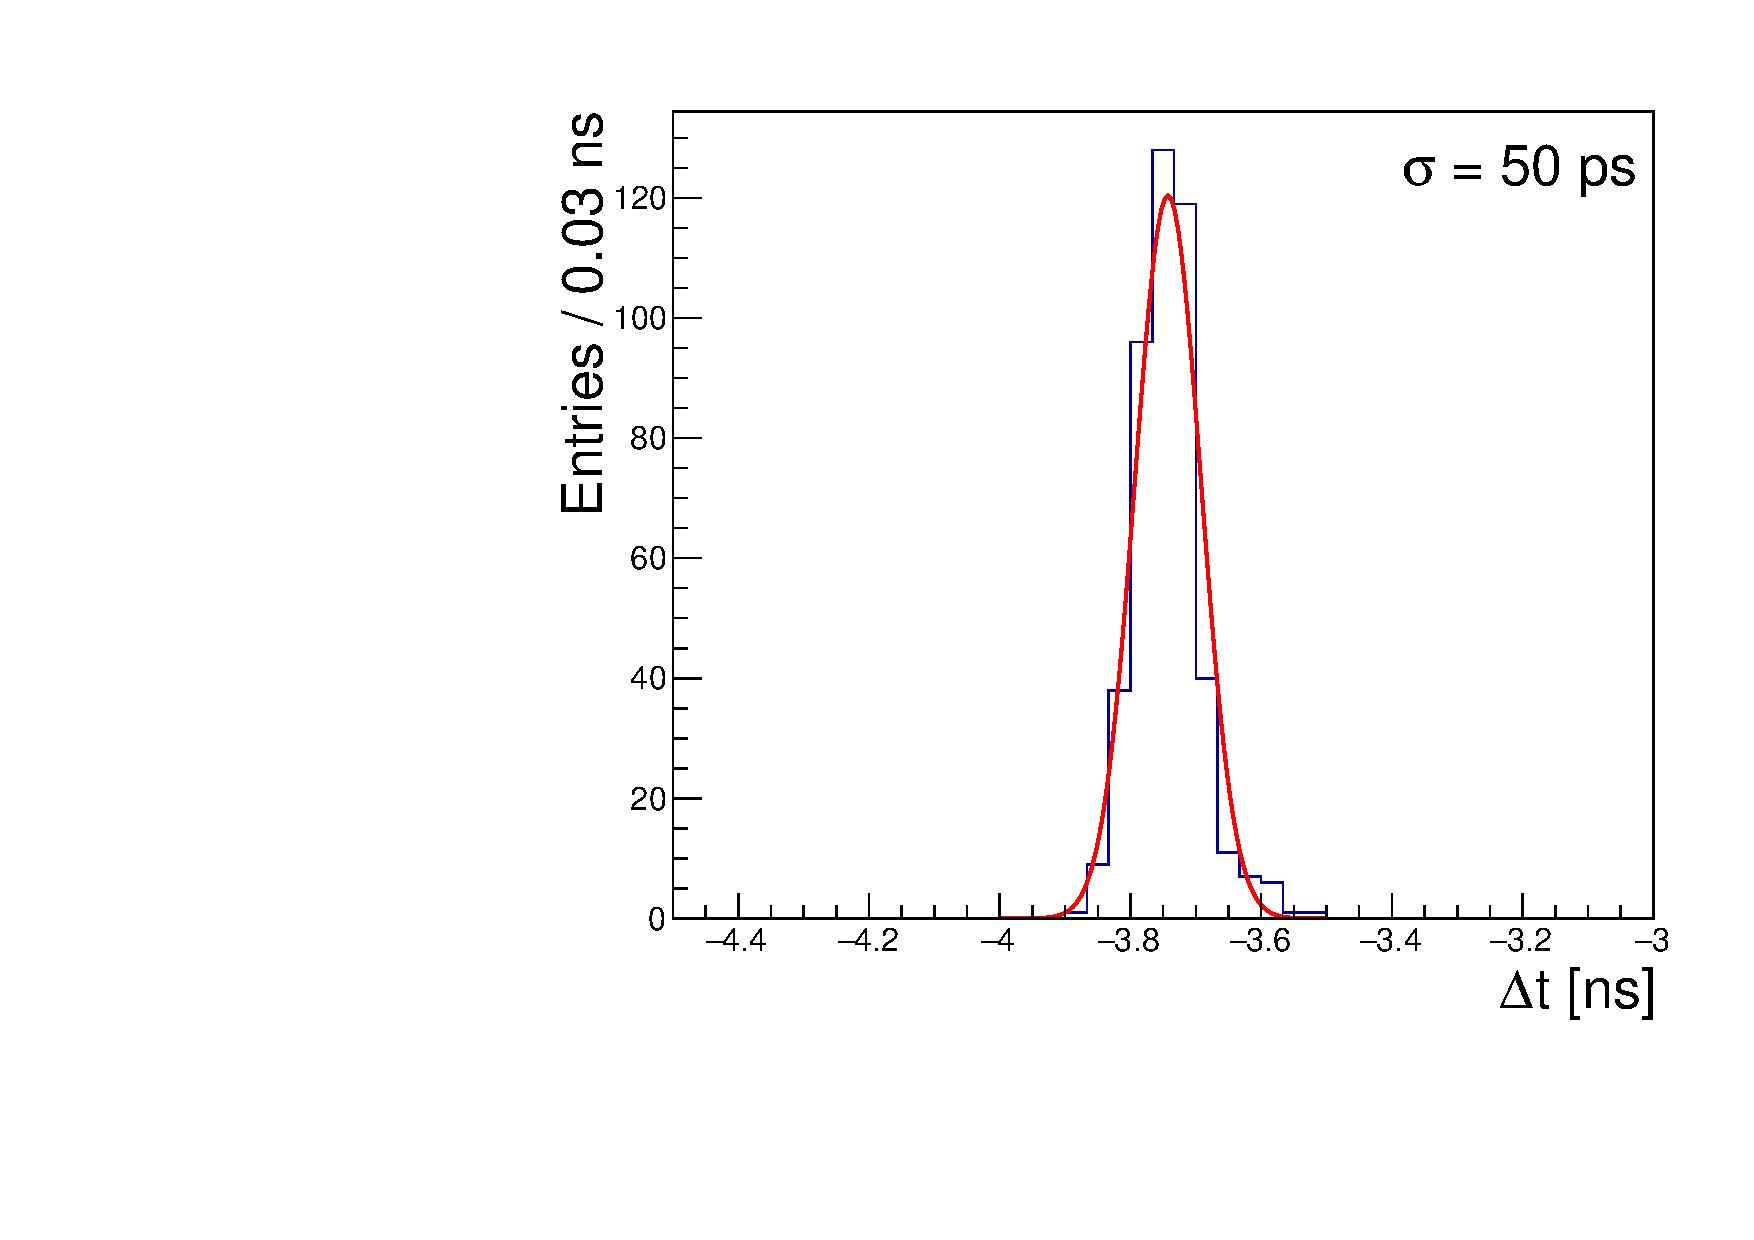
\includegraphics[width=8cm]{Images/exdt/exdtWI.pdf}
	\caption{\small Example $\Delta t$ histograms and resulting time resolution. Left: time resolution for one run using the naive highest-signal-integral pixel time stamp algorithm. Right: time resolution for the same run using the better weighted multiple pixel time stamp algorithm.}
	\label{fig:exdt}
\end{figure*}

\title{\large}{\textbf{Discussion and Conclusion}}




\renewcommand{\refname}{\textbf\selectfont\normalsize References}
\begin{thebibliography}{9}
\bibitem{}

\bibitem{}


\bibitem{}


\bibitem{}


\end{thebibliography}

\title{\large}{\textbf{Acknowledgments}}



\end{document}
